\documentclass[binding=0.6cm, oneside]{sapthesis}%remove "english" for a thesis written in Italian
%Bachelor's (laurea triennale) thesis : Lau
\usepackage[english]{babel} %use this package for a thesis written in Italian
\usepackage[utf8]{inputenx}
\usepackage{indentfirst}
\usepackage{microtype}
\usepackage{amsmath}
\usepackage{amssymb}
\usepackage{float}
\usepackage{titlesec}
\usepackage{lettrine}
\usepackage{caption}
\usepackage{subcaption}
\usepackage{listings}
\usepackage{adjustbox}
\usepackage[toc,page]{appendix}
\linespread{0.9}
\usepackage[nottoc, notlof, notlot]{tocbibind}
%\onehalfspacing
%\counterwithout{footnote}{chapter}
\usepackage{hyperref}
\hypersetup{		
			colorlinks=true,
			linkcolor=red,
                        linktoc=page,
			anchorcolor=black,
			citecolor=red,
			urlcolor=blue,
			pdftitle={Analysis of fuzz testing campaigns (temp)},
			pdfauthor={Matteo Sabatini},
			pdfkeywords={thesis, sapienza, roma, university}
}

%Defining macros for comments
\usepackage{xcolor}
\usepackage{xspace}
\newcommand{\mytext}[2]{\textcolor{#1}{#2}}

\newcommand{\tofix}[1]{\mytext{red}{#1}}

\newcommand{\mynote}[2]{\xspace\fbox{\bfseries\sffamily\scriptsize{#1}}
	{\small$\blacktriangleright$\textsf{\scriptsize\emph{#2}}$\blacktriangleleft$}}
\newcommand{\matteo}[1]{\mytext{magenta}{\mynote{MM}{#1}}}
\newcommand{\ziosaba}[1]{\mytext{cyan}{\mynote{ZS}{#1}}}


\title{Detecting Overlooked Bugs in Autonomous Fuzzing's Campaigns (for Open-Source Projects)(temp)}
\author{Matteo Sabatini}
\IDnumber{1794627}
\course{Cybersecurity}
\courseorganizer{Facolt\`a di Ingegneria dell'informazione, informatica e statistica}
\submitdate{2023/2024}
\copyyear{2024}
\advisor{Prof. Daniele Cono D'Elia}
\coadvisor{Dott. Matteo Marini}
\authoremail{sabatini.1794627@studenti.uniroma1.it}
\examdate{(??)}
\examiner{Prof. ??} \examiner{Prof. ??} \examiner{Prof. ??}  \examiner{Prof. ??}  \examiner{Prof. ??} \examiner{Prof. ??}  \examiner{Prof. ??}
\thesistype{Master thesis}

%we refer to http://ctan.mirrorcatalogs.com/macros/latex/contrib/sapthesis/sapthesis-doc.pdf for an exhaustive description of the sapthesis documentclass.






\begin{document}


\setlength{\parindent}{0pt}    %elimina l'indentazione leggermente a destra per ogni nuovo capitolo/paragrafo
\frontmatter
\maketitle

\begin{acknowledgments}
non so mai che scriverci :(
\end{acknowledgments}


\begin{abstract}
\matteo{Don't use random newpages and newlines; let sapthesis do its things. Use double newlines (intendo il tasto invio, non il comando) instead of the command newline, or are you using it for some specific reason?}
\ziosaba{For the "newline", I use them mainly because they give me visual clues on how much spacing I'm putting between paragraphs. I usually put a single newline for the sake of readibility, as I don't really like wall of texts, or when there is a weird spacing between words for the justification. A double newline means that the two paragraphs are connected but leave some space for the reader. A triple newline usually means that the next paragraph talks about a different topic or is not directly related to the previous one.}
\ziosaba{For the "newpage", again it's just a visual clue to make sure that the next paragraph that I'm writing will be on the next page. I used it situations where just the first one or two lines from the next paragraph were at the bottom of the page and the remaining 99\% was on the next one, for the sake of continuity.}
\end{abstract}




\tableofcontents


\titleformat{\chapter}[display]  
{\normalfont\Huge\bfseries}{\chaptertitlename\ \thechapter}{20pt}{\huge}  
\titlespacing{\chapter}{0pt}{0pt}{0pt}  

\mainmatter




\chapter{Introduction}
\ \\
Nowadays, technology has permeated every aspect of the human life, allowing everything and everyone to be interconnected anywhere and at any moment. Thanks to its importance, it quickly became one of the most popular field of work in the modern age, and it is now common for organizations to employ various technologies to provide their services. Because of this, cyber-crime also became very common.
\newline
The Cybersecurity is an aspect of informatics whose role is to ensure the safety of the technologies available and the people that are using it, both in terms of software and infrastructure. In this context, software testing and security play an important role to protect systems against security issues and vulnerabilities that could be potentially exploited by malicious people.
\newline \newline
Among the many approaches to software testing, \textit{fuzzing} is a very old technique invented in 1988, primarily used to automate simple tests that would have been otherwise performed by humans, that over the years gained popularity due to its ability to discover crashes and bugs in a program via extensive testing sessions. Although its concept it relatively easy, as it revolves around feeding random inputs to a program, it's effectiveness and simplicity of use allowed developers from all languages and level of knowledge to improve the security of their software.
\newline
Thanks to this technique, one of the most famous and critical bugs in history was discovered, the "Heartbleed" bug that affected OpenSSL.
\newline \newline
Since 2001, with the rise of "Open-Source Software", ensuring the security of software that was freely available and modifiable by anyone became a top priority: because the source code was freely accessible, it was only a matter of time before cyber-criminals began exploiting their vulnerabilities. Moreover, many modern paid applications often rely on such free software to provide their services. 
\newline
Given their popularity, Google announced the ClusterFuzz project in 2012, a cloud-based fuzzing infrastructure to test security-critical components of the Chromium web browser, where fuzzer developers could upload their own fuzz tool and collect bug-bounties if their product discovered a crash in the browser.
\newline
In 2016, this infrastructure was extended in a new campaign called OSS-Fuzz, allowing open-source developers to integrate their product in this ecosystem while Google provided its own infrastructure to perform continuous fuzzing of such projects.
\newline
Later, in 2021, Google announced yet a new project called FuzzBench, focused on helping the development of open-source fuzzers thanks to tests based on real-world benchmarks and daily reports.
\newline \newline
This work will focus on analyzing the campaigns previously mentioned, studying how they work and the results achieved, with the intention of highlighting not only their importance but also their shortcomings.




\newpage
\section{Context}
One of the 7 components in the "Software Development Life Cycle" (SDLC) is \textit{Testing}, which means analyzing and checking your code to make sure that it satisfies some quality, correctness and security criteria. This also provides crucial information that can be used to further improve the development of the product.
\newline
According to the "Consortium for IT Software Quality" (CISQ), poorly tested software cost the economy $\$2.08$ trillion dollars in 2020 alone \cite{forbes}, numbers that show how security against software bugs and vulnerabilities should be handled with maximum attention, especially considering also how most organizations now rely (almost) entirely on software technologies to provide their services across the globe.
\newline
Among the many goals of software testing, one of the most important ones is \textit{finding bugs}, defects in the code causing unwanted and unexpected results, that hinder the security of the product and may lead to vulnerabilities being exploited by malicious people.
\newline
In this context, one of the most commons approaches to finding bugs is \textit{automated testing}, that is using a tool to control the execution flow of the software being tested and analyze its results, and the automation derive from the fact that such tests usually involves repetitive tasks performed over long periods of time. This technique ensures fast and simultaneous execution of test cases with high reliability and consistency, as it its less prone to human error, the initial effort required for the initial set up is compensated by minimal maintenance requirements. Moreover, tests can be reused multiple times and integrated with different objectives in mind, including code coverage.
\newline
The technique used in this thesis is \textit{fuzzing}, an automated software technique based on repeatedly testing a software on different inputs with the intention of discovering crashes and other unwanted behaviors, especially ones that happen only when unusual conditions are met.
\newline
Specifically, all work was performed using the state-of-the-art fuzzer AFL++ \cite{AFL}.




\ \\
\section{Thesis Idea and Contributions}
This thesis revolved around analyzing and testing the effectiveness of automated testing infrastructures, more specifically the OSS-Fuzz and FuzzBench campaigns.
\newline
Given the organization running them and therefore the magnitude of such infrastructures in terms of projects tested, computing capabilities and time spent testing, one could expect these systems to accurately analyze programs and identify all possible bugs: in reality, reproducing the tests locally using the available corpora not only showed many bugs that were not being actively reported, but also that some of them shouldn't even be publicly accessible due to the extremely vulnerable errors they were causing.
\newline
This resulted in a study that focused on (re)testing some selected projects with the objective of discovering bugs, that would then be promptly reported to the respective developers hoping that this would help them make their software more secure. 
\newline
While their effectiveness and importance in software development remains undisputed, this work will show that the methodology used still managed to discover many bugs overlooked by these automatic systems, providing also some hypothesis regarding why this happened and how it could be fixed.




\newpage
\section{Outline}
The thesis will be structured as follows.
\newline
Chapter \ref{chap_2} introduces all the necessary concepts to understand what is fuzzing and how a fuzzer works, along with notions about some tools that are widely used in this field. It also introduces the definition of "Open-Source Program" and the infrastructures used in this work to perform fuzzing.
\newline
Chapter \ref{chap_3} discusses all the operations related to setting up the environment for the tests, the selection of the projects and how tests were performed, including the problems faced during this process and the solutions found.
\newline
Chapter \ref{chap_4} shows the results obtained, analyzing their importance, as well as discussing the reports issued and the developers' responses.
\newline
Finally, chapter \ref{chap_5} presents some final considerations about fuzzing, how it's perceived in the current era and provides some insights and suggestions on how to improve the current infrastructure.
\newline \newline \newline
\ziosaba{Chapter 5 outline to revise later}

\chapter{Background} \label{chap_2}
\ \\

This chapter will provide all the necessary background information and techniques employed in this thesis.
We will start by explaining the concept of \textit{fuzz testing}, with an in-depth analysis of how it works, the main components of a fuzzing session, and the different approaches available.
Follows an introduction on software sanitizers, highlighting their relevance in the context of fuzzing.
Then, we provide a short definition of "Open-Source Software", the main challenges faced during its development, and its connection with fuzzing in the modern era.
Concludes a thorough description of the modern automated testing infrastructures analyzed by this work, detailing their inner working and shortcomings.







\section{Fuzz Testing}
One of the most popular approaches to testing a program is \textit{automated testing}, where developers rely on scripts and specifications passed to external software or a created toolkit that automatically performs tests over long periods of time without human supervision. It can be divided into \textit{static testing}, which is based on a thorough analysis of the source code and uses techniques like symbolic execution to abstract the program execution, and \textit{dynamic testing}, which aims to execute the program many times with the objective of traversing all possible execution paths. It is particularly useful to formalize repetitive tasks into automated operations with high scalability, accuracy, consistency, and fast execution times. Additionally, programmers may prepare and use such pre-programmed tools with minimal costs after an initial effort in developing them, making it a crucial integration for large codebases and making sure that the product meets quality standards before being released. However, manual evaluation is still required and irreplaceable, both to ensure the correctness of the operations performed as well as to maintain and keep these tools effective and up to date with the software development \cite{automated_testing}.  

Among dynamic automated testing techniques, \textit{fuzz testing} (or \textit{fuzzing}) has become increasingly popular and widespread due to its ability to trigger critical issues such as crashes, assertions, memory leaks and undefined behavior, done by systematically testing the program using random, malformed and unexpected inputs. This allows developers to test their programs for so-called "corner-cases", i.e. situations that are difficult or complex to reproduce when the program is being properly used, but that could lead to unexpected and/or unwanted behavior potentially exploitable by malicious people and therefore should be handled properly. It also provides great flexibility, as this technique can be applied to an entire binary or selected small portions of code, introducing specific testing functions.

\newpage
We define 3 types of fuzz testing:
\begin{itemize}
    \item \textbf{application fuzzing:} used for UI elements (such as buttons, input fields) or command-line programs, tests may include high-frequency inputs, providing random/invalid content and inputs exceeding the expected size
    \item \textbf{protocol fuzzing:} used to test the behavior of network elements and servers when invalid messages are sent over a chosen protocol, useful to ensure that such content is not misinterpreted and potentially executed as commands
    \item \textbf{file format fuzzing:} used for programs that accept "structured inputs", i.e. files that have a precise and standard format (like .doc, .jpg), whose structure and content are altered to trigger unwanted behavior
\end{itemize}

The main concept of fuzzing revolves around testing a program on many (seemingly) random inputs over several \textit{fuzzing sessions}, each time discovering a bit more about the structure of the program, and then using this knowledge to create new testcases that attempt to trigger previously unseen execution paths and bugs: when an unexpected behavior is observed (i.e. crash, assertion, bugs, ...), the related input is reported to the user and saved for bug analysis, described in the following paragraphs. 
Each fuzzing session usually takes several hours or days to produce meaningful results; however, because this technique is mostly based on randomness, it also means that results may vastly differ between sessions, even across tests using the same configuration and resources. For this reason, multiple sessions are necessary before a conclusion regarding the safety of the program can be reached.

One of the most popular techniques to determine whether a particular test case was useful or not towards the final results is to analyze \textit{code coverage}: this metric represents a percentage that defines how much of the source code has been executed during a single fuzzing session, with the assumption that a high value means that most of the code has already been explored and there is a lower chance of having undetected bugs coming from already tested execution flows.
\begin{figure}[h]
\makebox[\textwidth][c]{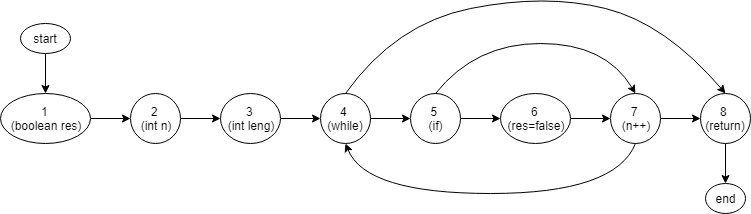
\includegraphics[width=0.67\paperwidth]{foto/cfg.png}}
\caption{CGF taken from a sample binary provided as input to IDA Disassembler \cite{ida}}
\label{fig:cfg}
\end{figure}


\newpage
This is usually done by creating a "Control Flow Graph" (CFG) of the program, i.e. a representation in graph notation of all paths available during a single execution flow: each node in the graph represents a "basic block", i.e. a sequence of instructions or statements with no jumps, and the edges between nodes represent jumps, loops and branch construct (if-else) in the program's execution (see figure \ref{fig:cfg}). By analyzing a single execution flow and measuring the number of nodes and edges traversed, the number of functions triggered, and which branches were activated during conditional statements, the fuzzer keeps track of all paths that have yet to be explored, providing useful information when generating new testcases. 

Therefore, we define \textit{interesting input} as any testcase that increases the code coverage achieved in a fuzzing session, and it is used as a reference when generating new testcases to hopefully get even more coverage.


\subsection{What is a fuzzer}  \label{fuzzers}
A \textit{fuzzer} is the tool performing fuzz testing, taking as inputs the program being tested and a set of testcases that will be used during the fuzzing session. It is responsible for executing the program against all the provided inputs in an automated manner, analyzing each execution for potential unwanted behavior, and producing new and useful testcases for future fuzzing sessions that will attempt to trigger new execution flows and even more bugs.
\begin{figure}[h]
\centering
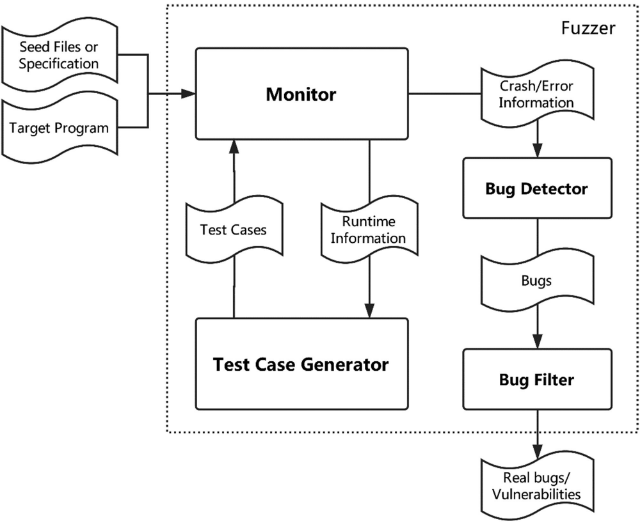
\includegraphics[scale=0.46]{foto/fuzzing_workflow.png}
\caption{General fuzzing workflow \cite{fuzzing_survey}}
\label{fig:fuzzing_workflow}
\end{figure}

In general, a fuzzer is composed of the following key elements \cite{afl_docs} \cite{fuzzing_survey}.

\textbf{Target program.}\ \ \ Refers to the program that is being evaluated: it could be either binary or source code, although source code of real-world software is usually not accessible.

\textbf{Program's Specification.}\ \ \ Some fuzzers can receive as input the program's specification, a formal description of the target program and its behavior using as reference the available documentation and source code, which translate its functionalities and expected behavior using a specific grammar that the fuzzer understands. However, this information is rarely available and often too difficult to infer without the appropriate data.

\textbf{Observer (or Monitor).}\ \ \ Provides runtime information observed during the execution of the target to the fuzzer, leveraging techniques such as code instrumentation, taint analysis, code coverage, and many more. Such information may be relatively simple, like the total running time for a test and its output, to more advanced ones, like the maximum depth of the stack. They are usually not preserved across executions unless an "interesting input" is encountered, in which case they are relayed to the \textit{Test case generator} to be used as reference during the generation of new testcases. 

\textbf{Executor.}\ \ \ Responsible for defining how the program will be executed and the arguments passed on each run. The input for a single test is provided either by writing it in some specific memory location or passed as argument to a so-called "harness function", although each fuzzer has its own implementation of this element. Given this, we briefly mention a few standard functionalities that compose this element. The \textit{InProcessExecutor} runs the "harness function" and provides crash detection. The \textit{ForkServerExecutor} is responsible for spawning different child processes to fuzz. The \textit{TimeoutExecutor} wraps and installs a timeout for another running executor.

\textbf{Test case generator.}\ \ \ Performs generation of new testcases to increase code coverage using runtime information received from the observer and \textit{interesting inputs} as reference. This can be done using either \textit{mutation} or \textit{generation}, depending on the type of fuzzer chosen (discussed later), although it is important to note that there is no one-size-fits-all solution.

\textbf{Feedback.}\ \ \ Chain of components that classify the result of a single execution and determine if the initial input is "interesting" or not analyzing the information received from the observers and the updated coverage map. Some examples shown in Figure \ref{fig:fuzzing_workflow} are the \textit{Bug Detector}, which collects and analyzes debug information during crashes and errors, and the \textit{Bug Filter}, which classifies the errors collected.
Each component of this chain usually has its own objective (crashes, timeouts, new execution flows discovered, assertions), and combining them in boolean expression allows the developer to collect more fine-grained results and maximize a desired target function.

\textbf{Testcase.}\ \ \ Data taken from an external source and provided as input to the tested program to observe its behavior, usually in the form of bytes arrays. Each testcase is defined by a set of metadata like ID, description, and expected results. The first fuzzing session takes a set of inputs defined and provided by the developer itself, while future fuzzing sessions will also rely on previously discovered "interesting inputs". 

\textbf{Corpus.}\ \ \ Location where testcases are stored, usually disk or memory. An \textit{input corpus} may be composed of several testcases with the same properties, like crashing the program under a specific situation. An \textit{output corpus} is composed of all testcases that are considered "interesting" or a collection of all inputs that triggered a bug in the program.


\newpage
Fuzzers can be then categorized using the 3 following characteristics.

\textbf{Input generation.}\ \ \ During each fuzzing session, one of the most important operations performed by the fuzzer is the generation of new testcases, with the objective of diversifying and increasing the effectiveness of the corpora that will be used on future fuzzing sessions: more specifically, an effective fuzzer should be capable of generating inputs "valid enough" so that they are not rejected from the program's parsers, but also "invalid enough" to potentially trigger corner cases. Given this, we distinguish between \textit{mutation-based} and \textit{generation-based} fuzzers. The \textit{mutation-based fuzzers} require an initial seed of inputs as reference, and the generation of new inputs is performed by applying "mutators" on the provided seeds: these operations range from flipping/adding/removing bits (or bytes), performing mathematical operations and sometimes even completely randomizing its content. Finally, these mutations are usually mixed forming sequences to increase randomness. The \textit{generation-based fuzzers}, instead, rely on a good source of randomness to generate new inputs from scratch, and for this reason they do not depend on the existence of a good initial corpus nor its quality, although they require more starting time before the tests become effective.

\textbf{Input's structure awareness.}\ \ \ Another information useful to the fuzzer, although not always available, is the "input model", i.e. the correct structure that a file must have when testing programs that follow rigorous standards. However, not all of them provide this feature, and for this reason we define \textit{smart} and \textit{dumb} fuzzers.
A \textit{smart mutation fuzzer} might leverage this knowledge to switch between different types of inputs, while a \textit{dumb mutation fuzzer} can only rely on the structure of the "interesting inputs" and apply limited random mutations, usually resulting in a much lower proportion of valid inputs being generated.
A \textit{smart generation fuzzer} uses this information to avoid wasting resources on generating inputs that are too random to be accepted, as the \textit{dumb generation fuzzer} attempts to generate new inputs without any reference, oftentimes putting more stress on the program's parser rather than the program itself due to the overwhelmingly high number of invalid inputs generated in the first phases.

\textbf{Program's structure awareness.}\ \ \ Fuzzers may be accompanied by program analysis techniques to increase the efficiency and effectiveness of the tests. A \textit{black-box fuzzer} is completely unaware of the program's structure, therefore assumes the program as a simple machine that takes a random input and generates an according output: this approach is relatively fast, can be easily parallelized and has good scalability, however it will most likely find only bugs that do not require particular conditions to be met to be triggered, also called "surface bugs". A \textit{white-box fuzzer} employs program analysis techniques to systematically explore and reach critical program locations through meticulously crafted inputs, allowing you to discover bugs that could be potentially hidden deep in the program: while this approach is arguably the most effective one, it implies that bugs related to unknown aspects of the program can be easily missed, and the time used to analyze the program as well as generating such specialized input exponentially increases with the program's complexity.
A \textit{gray-box fuzzer} attempts to find a balance between efficiency and effectiveness by integrating the best aspects of both approaches: using a minimal amount of knowledge of the program's structure to achieve a sufficient degree of code coverage such that the results obtained are satisfactory.







\newpage
A \textit{fuzzing session} defines the process of testing a program using a fuzzing tool.
Assuming the program has been properly compiled using the chosen fuzzer, the first step is to simply start the fuzzing session and let the fuzzer execute the program on many different testcases. After some time, when either the initial corpus has been exhausted (mutation-based) or the fuzzer learned what is an acceptable input (generation-based), it starts applying random operations to generate new testcases. 

During each execution, code coverage and unexpected behaviors are tracked, so that all testcases that increase any of these statistics will be regarded as "interesting inputs" and saved in a separate queue. In this context, the fuzzer has to be sensible enough to distinguish between crashing and non-crashing inputs without having full knowledge over the program tested, and therefore \textit{sanitizers} are used to "instrument" the source code and inject assertions that make the program crash when a particular kind of failure is detected. Section \ref{sanitizers} explains this concept more thoroughly.

At the end of each fuzzing session, the user is presented with three results: a collection of statistics regarding the coverage achieved and bugs found, a list of inputs that caused crashes along with some metadata (testcase ID, bug type, memory state, etc...), and a set of "interesting inputs" that can be used in future fuzzing sessions to provide the fuzzer with even more information about the structure of a good input that explored the deepest parts of the program. 
The statistics provided may be useful to understand how effective this particular fuzzing session was with respect to the previous ones, if the initial corpus needs to be refined, and whether the changes applied to the code have been fruitful or not.
The new set of "interesting inputs" is then added to the existing initial corpus, which in turn is \textit{pruned}: this process removes any duplicates and inputs that trigger the same execution flow or bugs, which is crucial to ensure that the size of the corpus does not explode over time.
Finally, the developer has to analyze all the inputs that caused a bug and perform \textit{bug triage}: execute each input individually to observe its output, determine which kind of error occurred and why, fix the bug entirely (if possible) or at least patch the problem, and ensure that the bug does not occur in future fuzzing sessions by including the triggering input(s) in the set used for the tests.

All these steps are repeated across many different fuzzing sessions, sometimes even changing the scope of the tests to increase code coverage or stressing the program with buggy inputs, each time making the program more secure against vulnerabilities and more robust to extraneous inputs. 

In conclusion, many modern fuzzers originate from a solution that represented a breakthrough in fuzzing research called \textit{American Fuzzy Lop} (also known as \textit{AFL} \cite{afl}), a "dumb mutation-based fuzzer" that achieved many results over the years: in September 2014 it discovered "Shellshock" \cite{shellshock} (also known as "Bashdoor"), a family of security bugs affecting the Unix Bash shell that allowed malicious users to execute arbitrary commands without confirmation, while in April 2015 it discovered the famous "Heartbleed" \cite{heartbleed} bug in OpenSSL, which allowed malicious users to decipher the otherwise encrypted communications used by the TLS protocol.
Since 2017, when the development of this tool was stopped, there have been many variants and improvements of this tool, and some honorable mentions are WinAFL \cite{winafl}, VUzzer \cite{vuzzer}, FairFuzz \cite{fairfuzz}, Fuzzolic \cite{fuzzolic} and QSYM \cite{qsym}. This thesis focused on AFL++ \cite{AFL++}, a direct fork of AFL with new and better mutation and coverage algorithms, which is the current state-of-the-art fuzzer.










\newpage
\section{Sanitizers} \label{sanitizers}
A \textit{code sanitizer} is a tool used to detect bugs in a program during both compilation and runtime, with different sanitizers specializing in detecting various kinds of bugs: misuse of addresses, stack- and heap-overflows, use of uninitialized memory, memory leaks, and undefined behavior.

They are added to a program through "instrumentation", which refers to modifying either the source code or the binary code to introduce some additional functionalities and references that can be used by other tools to perform code analysis, logging, and profiling. Although code sanitizers should be a standard practice in the development cycle of a program, introducing these tools requires knowledge and extensive tests to check for potential errors, also because they do not always interact very well with shared libraries or other external dependencies. It is also extremely important to mention that these bug detection tools are not meant to be linked against production executables, as their runtime was not developed with security-sensitive constraints and may compromise the security of the released product \cite{asan_docs}\cite{msan_docs}\cite{ubsan_docs}.

A \textit{compile sanitizer} is a tool that performs instrumentation at compile-time, meaning that it introduces functions and libraries that will be then added and compiled together with the original source code, effectively altering its default behavior. Their advantages are twofold: they are able to achieve full coverage and provide warnings and errors during the compilation process, since the analysis is performed directly on the source code and includes all possible paths, and they are also able to detect errors during the execution of the program, although limited by the single execution flow analyzed. However, these sanitizers introduce a non-trivial overhead in terms of increased compile time, execution time, and memory usage, which may cause problems when it comes to managing computing resources.

A \textit{binary sanitizer} is a dynamic binary instrumentation (DBI) framework that performs "Just-in-Time" (JIT) compilation to introduce additional instructions and analysis callback during the execution of a program, effectively without modifying the original code, and they often rely on dynamic binary analysis (DBA) tools to analyze programs at run-time at the level of the machine code. Also, these sanitizers are dependent on the input given and the resulting execution flow analyzed, therefore they are not capable of achieving full code coverage. Moreover, this analysis requires attaching another external process to instrument the original one, which usually causes massive slowdowns and sometimes might even break the original's code functionality.

This work focused on using several compile sanitizers developed by Google \cite{san_repo} as part of its tool suit provided to open-source developers, along with a popular binary sanitizer \cite{valgrind_web} to perform a cross-check on the results produced by the compile sanitizers, as these tools have been proven to be particularly effective when combined with fuzzing due to their ability to trigger bugs.




\newpage
\subsection{ASan and LSan}
The \textit{Address Sanitizer} \cite{serebryany2012addresssanitizer} is a memory error detection tool for C/C++ that helps developers to find and fix any out-of-bounds accesses to heap, stack and global objects, use-after-free bugs and provides protection against stack-based and heap-based overflow, making it one of the most popular and effective sanitizers.

When allocating bytes for a buffer and performing an access beyond such boundaries, a program will usually crash with an "out-of-bounds exception", but it could also happen that it is valid to access information in the unallocated address, in which case the program will crash unexpectedly and make it difficult for the developer to understand the problem. Moreover, if such addresses are not properly freed, they could leave a so-called "dangling pointer", and thinking that this memory location still holds valid data (maybe even confidential one) implies serious security issues.
If an attacker discovers a program with such vulnerabilities, he could use them to crash the application, corrupt or retrieve sensitive data, or even perform a "remote code execution" attack by inserting some malicious code via this buffer overrun and causing the program to jump and execute that particular memory location, creating an attack vector where anything is possible. 

To prevent this, the sanitizer uses a shadow memory to map the memory regions allocated by the application and record whether each byte of such areas can be safely accessed by load/store operations. Each memory region is assigned a shadow counterpart, containing metadata about its size and the offset range that can be used to safely access it, while any attempt to read/write beyond such boundaries will trigger a sanitizer error, as shown by the figure below:

\begin{figure}[h]
\centering
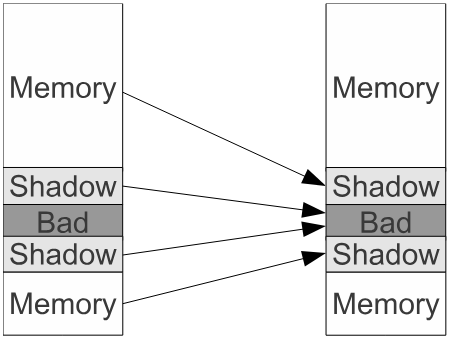
\includegraphics[scale=0.6]{foto/shadow_memory.png}
\caption{Memory mapping of ASan \cite{serebryany2012addresssanitizer}}
\label{fig:asan_shadow}
\end{figure}

Detection of out-of-bounds accesses to global variables and stack objects is done in a similar way, i.e. by creating poisoned memory regions around such objects: \textit{global variables} are poisoned at compile-time and their addresses computed during the application startup, while \textit{stack objects} are poisoned and recorded at run-time.

The management of the shadow memory is done by ASan run-time library, containing a specialized implementation of the \verb|malloc| and \verb|free| functions which allocate extra memory for shadow and poisoned memory zones as well as keeping a FIFO stack of allocated and freed memory regions to detect use-after-free, double-free and invalid-free bugs.

This sanitizer is also provided with another component called \textit{Leak Sanitizer} (or \textit{LSan}), a memory leak detector enabled by default that returns which portions of the program are leaking memory as well as the size leaked, thanks to comprehensive and exhaustive stack traces. A memory leak is a condition where a program fails to release memory that is no longer needed due to developers' negligence or software error, effectively reducing the amount of memory available by the machine, and this will inevitably lead to performance degradation (trashing). Although this component may seem very helpful, it usually generates huge logs especially when having complex programs that heavily rely on external libraries, which oftentimes do not perform clean releases of the objects used.

Finally, ASan adds a slight overhead, increasing execution times by an average of 170\% and memory usage by 3.4x \cite{serebryany2012addresssanitizer}.





\subsection{MSan}
The \textit{Memory Sanitizer} \cite{stepanov2015memorysanitizer} is a memory reads detector for C/C++ that helps developers to find and fix use-of-uninitialized-memory (UUM) bugs, which are considered to be quite tricky as they do not necessarily occur in every execution and could be triggered by any operation performed by the program. The C/C++ languages leave memory management to the developer, who is responsible for correctly allocating, using, and freeing every memory region that is accessed by the program, and for this reason they are also defined to be "memory-unsafe": in fact, unless specified, any new allocation operation performed by these languages creates uninitialized stack and heap objects. Such vulnerabilities may not only be exploited to alter the execution flow and inject malicious code, but also to leak information about a program's internal stake, such as the content of the stack or heap.

A UUM bug usually originates from any operation that loads a value from an uninitialized memory region, resulting in an \textit{undefined value} being returned, and operations like conditional branch, syscalls, and pointer dereference are most likely to trigger them. This sanitizer works by using a shadow memory to map each bit of application memory and encode its state (0 initialized, 1 otherwise): all newly allocated memory is poisoned, i.e. the corresponding shadow memory is initialized to \verb|0xFF|, and "shadow propagation" operations are performed to safely copy an uninitialized variable to different memory regions as well as safely perform simple logic and arithmetic operations on them without occurring in errors.

\begin{figure}[h]
\centering
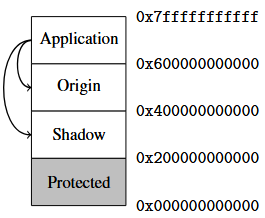
\includegraphics[scale=0.8]{foto/shadow_memory_2.png}
\caption{Memory mapping of MSan \cite{stepanov2015memorysanitizer}}
\label{fig:msan_shadow}
\end{figure}

Given that UUM bugs are notoriously hard to reproduce and debug, MSan provides the "origin-tracking-mode" to obtain more comprehensive and descriptive stack-traces. If necessary, there is also the "advanced-origin-tracking-mode", which records the entire stack and all operations that happen between the allocation and load of uninitialized variables, but its usability is still discussed due to the huge amounts of memory it requires.

The management of the shadow memory is done by MSan run-time library, which maps the "shadow" and (optional) "origin" areas and marks as uninitialized any new allocated regions as well as the deallocated ones. To update the shadow region, a large subset of the standard \verb|libc| functions are intercepted.

Fixing these bugs generally requires little to no effort, but many developers avoid this sanitizer due to the huge slowdown that it introduces. In fact, MSan increases execution times by an average of 300\% and memory usage by 2x on short programs, values that rapidly worsen with complex programs \cite{stepanov2015memorysanitizer}.





\subsection{UBSan}
The \textit{Undefined Behavior Sanitizer} \cite{ubsan_docs} is a fast undefined-behavior detector for C/C++ that helps developers to find and fix undefined-behavior (UB) bugs. The C language specification allows developers to perform many complex and (sometimes) unreasonable operations on the assumption that they know what they are doing, and this leads to the compiler making arbitrary decisions when the code does not conform to some expected values: for example, an array indexed with an out-of-bound value will not always crash the program if said memory location contains valid content that belongs to the program, while performing a conversion between two data types of different sizes will result in unpredictable loss of data due to rounding operations. This means that different compilers will handle such situations differently and produce unexpected results each time they are executed, all without taking into account that the hardware used and the level of optimization chosen will also affect these results.

Common operations that may lead to undefined behaviors are: array subscription out of bounds, overflows/underflows of numerical types due to mathematical or logical operations, shifts of numerical values, dereferenced, misaligned or null pointers, and invalid conversions between data types. Although this list is not exhaustive of all possible scenarios, it is apparent that most of the problems mentioned could be fixed with negligible effort and avoided altogether by applying appropriate coding standards.  

This sanitizer works similarly and sometimes overlaps with ASan, putting protected regions around buffers and inserting correctness-checking functions after all mathematical, logical, and implicit/explicit cast operations. By default, due to its simplistic nature, the tool does not print stack-traces and uses a minimal run-time library, although the "print-stacktrace-mode" option can be enabled to obtain more comprehensive results.

To conclude, UBSan adds a trivial overhead, increasing execution times by an average of 120\% and memory usage by 2x \cite{ubsan_docs}.



\subsection{Valgrind}
\textit{Valgrind} is a Dynamic Binary Instrumentation (DBI) framework for building dynamic analysis tools, i.e. tools that perform code analysis at runtime and capable of achieving full coverage of user-mode code. It is distributed with seven production-quality tools that perform code profiling, memory analysis, and threading bugs, with similar functionality to ASan and MSan \cite{valgrind_web}.  

The tool relies on dynamic binary recompilation to load the client program into the "Valgrind Core" and (re)compile the client's machine code in small blocks using a "Just-In-Time" (JIT) approach, producing a so-called "Intermediate Representation" (IR) which is then instrumented with analysis code. This translated code is then stored in a code cache, so that it can be rerun when necessary avoiding this overhead. It is also capable of monitoring the CPU registers during the program execution by taking control of the real CPU and (conceptually) running the client program on a simulated one, and the concept of "shadow memory" is used to analyze and protect both memory and CPU registers \cite{Valgrind_1} \cite{Valgrind_2}.

This work relied on Valgrind's memory-analysis tool called \textit{Memcheck} \cite{memcheck_docs}\cite{memcheck_paper}, a memory-error detector for C/C++ program when performing accesses to heap and stack elements, use of uninitialized and undefined values, incorrect allocation and freeing of heap memory, misuse of allocation functions and finally tracking memory leaks. Since most of its functions overlap with MSan, it was used as a replacement for detecting UUM bugs when analyzing projects that relied heavily on external libraries: this is because, of the compile sanitizers mentioned above, MSan is the only one that requires all libraries linked to the executable to be rebuilt with this sanitizer to get meaningful results. However, this process proved to be too cumbersome and beyond the scope of this work, also because most projects used statically linked libraries rather than compiling them from scratch.

While Valgrind is a very popular and widely used tool, it also suffers from a major limitation due to its design choice, which is that it is a single-threaded program: this means that its execution cannot be parallelized and the entire program and its analysis run on a single CPU core and kernel thread. In fact, Valgrind applies an average slowdown of 4x by default, value that can range from 10x up to 100x for CPU-bound programs when other analysis tools are introduced \cite{Valgrind_1}: for example, the Memcheck tool introduces a slowdown between 20x-30x for most programs \cite{memcheck_docs}.





\newpage
\section{Open-Source Software} \label{opensource}
The \textit{Open-Source Software (OSS)} is a computer software developed in a collaborative and public manner, released under a particular license that allows other users to freely use, study, modify, and distribute the software and its source code for any purpose: this allows many users to actively participate in the development of a software by proposing changes and new improvements.
To be eligible as open-source software, the license's distribution terms must comply with several criteria \cite{osd}: the main concept is to let anyone easily download your program and access its source code, allowing them also to modify and redistribute the project without additional fees as long as the original code is appropriately credited. 

Given all this, one could argue that making all this information publicly available poses a real threat to security: history has shown us many times that, given enough time and resources, releasing the source code of a program will result in malicious users discovering bugs and vulnerabilities that could have potentially catastrophic consequences. 

For this reason, we mention some key aspects that should be considered when approaching open-source software.

\textbf{Development.}\ \ \ Open-source software is usually released under two development branches: a "stable" version, composed of all the functionalities that have been thoroughly tested and work as intended, and a "build" version, that is slightly buggier as it includes proposed changes and new features that have yet to be refined. Releasing the "build" version early not only allows the developers to showcase their work and attract even people, but also provides them with feedback from real users that are willing to run untested versions of their software.

\textbf{User interaction.}\ \ \ Providing full access to the source code means that other users might want to contribute to the program's development and help the developers in improving and refining the product: considering that each user may have different knowledge and programming skills as well as different testing environments, this allows them to test and benchmark the product on a wide range of systems, further increasing the probabilities of finding new and unknown bugs that may be specific to a single OS or architecture.

\textbf{Bug reporting.}\ \ \ Although any user has the right to mention a bug, error, or mistake in the program or the documentation, it is still up to the developers to ensure the truthfulness of what has been reported and how to tackle it. For example, bugs that are not security-relevant or that may be related to QoL aspects are easily pushed back as secondary problems or simply ignored altogether. Sometimes, if the developers are kind enough to accept your request but do not have time and resources to solve it, they might ask for a proposed fix and cite the user themselves in the next patch notes as a way of thanking them.



\newpage
\section{Continuous Fuzzing}
In the past decade, fuzzing became one of the most popular dynamic automated testing techniques, with both small and large companies employing it to discover bugs and vulnerabilities in their products. However, a fuzzing session needs to run for at least 24 hours \cite{evaluating_fuzz} to produce meaningful results, and time is a resource that most organizations cannot afford to lose. For this reason, they often employ short but continuous fuzzing campaigns together with a software development paradigm called \textit{CI/CD pipeline} (\textit{Continuous Integration} and \textit{Continuous Delivery}): CI refers to the practice of frequently integrating and testing changes to the source code to ensure that the product is always in a well-functioning state. CD is a delivery strategy in which software is developed in short tasks and released with incremental updates, helping developers to reduce costs by making development simple and repeatable, but also avoiding unnecessary risks from applying too many changes at once. 

In general, a continuous fuzzing framework refers to an automated framework that integrates any changes committed to the code, builds and tests debug versions of the program with one (or more) configuration of fuzzers and sanitizers, and finally deploys a new version of the product to end users. To further increase early defect discovery, many of these frameworks rely on a technique called \textit{ensemble fuzzing}, with a workflow similar to the one shown below:

\begin{figure}[h]
\makebox[\textwidth][c]{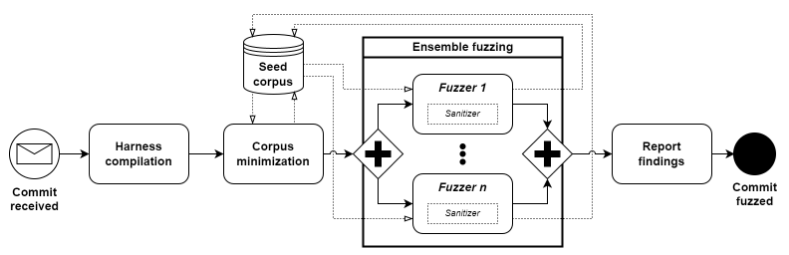
\includegraphics[width=0.75\paperwidth]{foto/ensemble_fuzzing.png}}
\caption{Generic design of ensemble fuzzing in a CI/CD pipeline \cite{continuous_fuzzing}}
\label{fig:continuous_fuzzing}
\end{figure}

Instead of focusing on testing a program with a single fuzzer (along with sanitizers) for several hours, this approach focuses on testing the same program in short sessions with different combinations of fuzzers and sanitizers, mixing and matching mutation-based and generation-based fuzzing tools. Each fuzzer runs asynchronously and separately from the others, collecting interesting inputs and applying its own operations to generate new inputs. Then, all results are collected and synchronized into a single queue for analysis and use in subsequent fuzzing sessions: this approach maximizes both the diversity of inputs used, as each fuzzer will be using testcases produced by other fuzzers, and the diversity of results, as each fuzzer will test code differently potentially leading to the discovery of new bugs. Of course, in order to use this technique, developers must compile and prepare the binaries accordingly.

\newpage
We briefly mention a few popular continuous fuzzing infrastructures. Microsoft announced in 2020 the \textit{Project OneFuzz Framework} \cite{onefuzz}, an extensible and open-source self-hosted fuzz testing framework with the goal of enabling developers to easily and continuously fuzz programs prior to their release while scaling fuzzing workloads in the cloud thanks to Azure. It allowed developers to build and compose a continuous fuzzing workflow using several fuzzing tools, perform automatic bug triage and results deduplication with multi-platform design in mind. Unfortunately, its development was stopped as of September 2023 \cite{onefuzz_repo}. GitLab provides continuous coverage-guided fuzz testing as part of its CI/CD services \cite{gitlab_fuzz}, supporting many different languages and fuzzing engines. Google provides \textit{ClusterFuzzLite} \cite{google_lite_repo}, a continuous fuzzing solution as part of CI workflows to fuzz pull requests and catch bugs before they are committed \cite{google_lite}, and \textit{OSS-Fuzz} \cite{ossfuzz_paper}, a continuous fuzzing service for open-source software.

Google was also one of the first major companies that connected automated testing, continuous fuzzing frameworks and open-source software together. The \textit{Google Open Source Project} \cite{google_oss} is a campaign started in 2004, one of the oldest open-source campaigns in the industry: it was initially meant to share Google-developed software under open licenses, with the intention of bringing free technology and information sharing to the public, but it quickly became a program dedicated to improving open-source ecosystems as a whole. Thanks to this campaign, many projects became popular and gained worldwide recognition such as Android OS, TensorFlow, the Go programming language, and many more.

This thesis will focus on two campaigns maintained by Google called \textit{OSS-Fuzz} \cite{ossfuzz_docs} and \textit{FuzzBench} \cite{{fuzzbench_docs}}: the first is a free platform that allows open source developers to fuzz their programs autonomously by integrating with existing CI/CD pipelines and relying on the computing resources provided by the Google Cloud Service, while the second allows fuzzer developers to test and improve their tools against real-world benchmarks thanks to automated testing and reporting. The objective was to evaluate a selected group of the projects that have been implemented in these repositories using alternative approaches, trying to discover bugs that will be then securely reported and disclosed to their developers in the hope of having them fixed.



\subsection{ClusterFuzz}
Before introducing the frameworks mentioned above, it is also important to define the underlying infrastructure. The \textit{ClusterFuzz Project} is a scalable fuzzing infrastructure with the objective of discovering security and stability issues in software through continuous coverage-guided fuzzing, it is also the main platform used by Google to test its products and the fuzzing back-end for \textit{OSS-Fuzz}. As of May 2023, it discovered over 25.000 bugs in Google proprietary software (e.g. Chrome) and 36.000 bugs with OSS-Fuzz \cite{clusterfuzz_docs}.

It is based on a highly scalable distributed system of VMs that performs fully automated fuzzing, bug triage, filing and closure of bug reports as well as providing performance statistics, and all operations are performed by two main components.
The \textit{App Engine} provides a web interface to the information collected during each fuzzing session, allowing the developers to easily access crashes, results, and other information. This is also where tests can be scheduled, which is done via \verb|cron| jobs.
The \textit{Fuzzing Bots Pool} is a cluster of VMs responsible for running the scheduled fuzzing sessions, and they perform the following operations:
\begin{itemize}
    \item \textbf{fuzz:} runs a fuzzing session, timeout different for each fuzzer
    \item \textbf{progression:} checks if a testcase still reproduces or if has been fixed
    \item \textbf{regression:} calculates the commits range in which a crash was introduced
    \item \textbf{minimize:} eliminates duplicate testcases from the input seeds
    \item \textbf{pruning:} minimize a corpus to the smallest size based on coverage information
    \item \textbf{analyze:} runs a manually uploaded testcase against a specific job to see if it crashes
\end{itemize}

\begin{figure}[h]
\makebox[\textwidth][c]{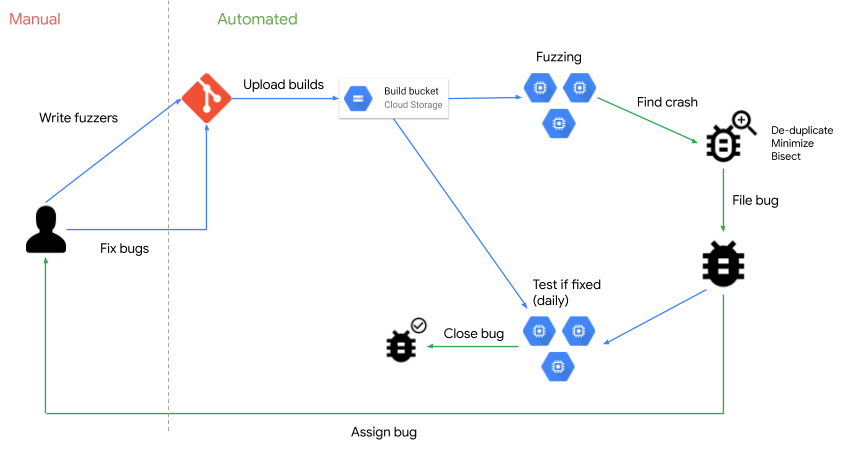
\includegraphics[width=0.64\paperwidth]{foto/clusterfuzz_architecture.png}}
\caption{ClusterFuzz main architecture visualized \cite{clusterfuzz_docs}}
\label{fig:clusterfuzz_architecture}
\end{figure}

Each VM performs these operations inside Docker instances created and uploaded by the developers, which are configured with all the tools and files necessary to correctly build and launch the fuzzing targets. Since some of these tasks are critical and should be treated as atomic operations, bots can be \textit{preemptible} or \textit{non-preemptible}: the former refers to a machine that can only run the "fuzz" task as it can be shut down at any moment, while the latter refers to a machine that is not expected to suddenly stop or crash and is therefore capable of performing all tasks.



\subsection{OSS-Fuzz}
The \textit{OSS-Fuzz Project} \cite{ossfuzz_paper} was founded in 2016 after the famous "Heartbleed" vulnerability was discovered in OpenSSL, one of the most popular open-source projects at the time for encrypting web traffic, as a response to provide developers with free fuzzing and private alerts services for their open-source projects. As of August 2023, it has helped identify and fix more than 10,000 vulnerabilities and 36,000 bugs in over 1000 projects \cite{ossfuzz_docs}.


While it was initially intended for languages that are not memory-safe (C/C++), it was later extended to provide support also for other popular languages such as Python, Go, Java, and Rust. Projects can be evaluated using several coverage-guided mutation-based fuzzing engines (such as LibFuzzer, AFL++ and Honggfuzz) in combination with Google Sanitizers (ASan, MSan and UBSan), while \textit{ClusterFuzz} acts as the back-end and provides bug reporting functionalities.

\begin{figure}[h]
\makebox[\textwidth][c]{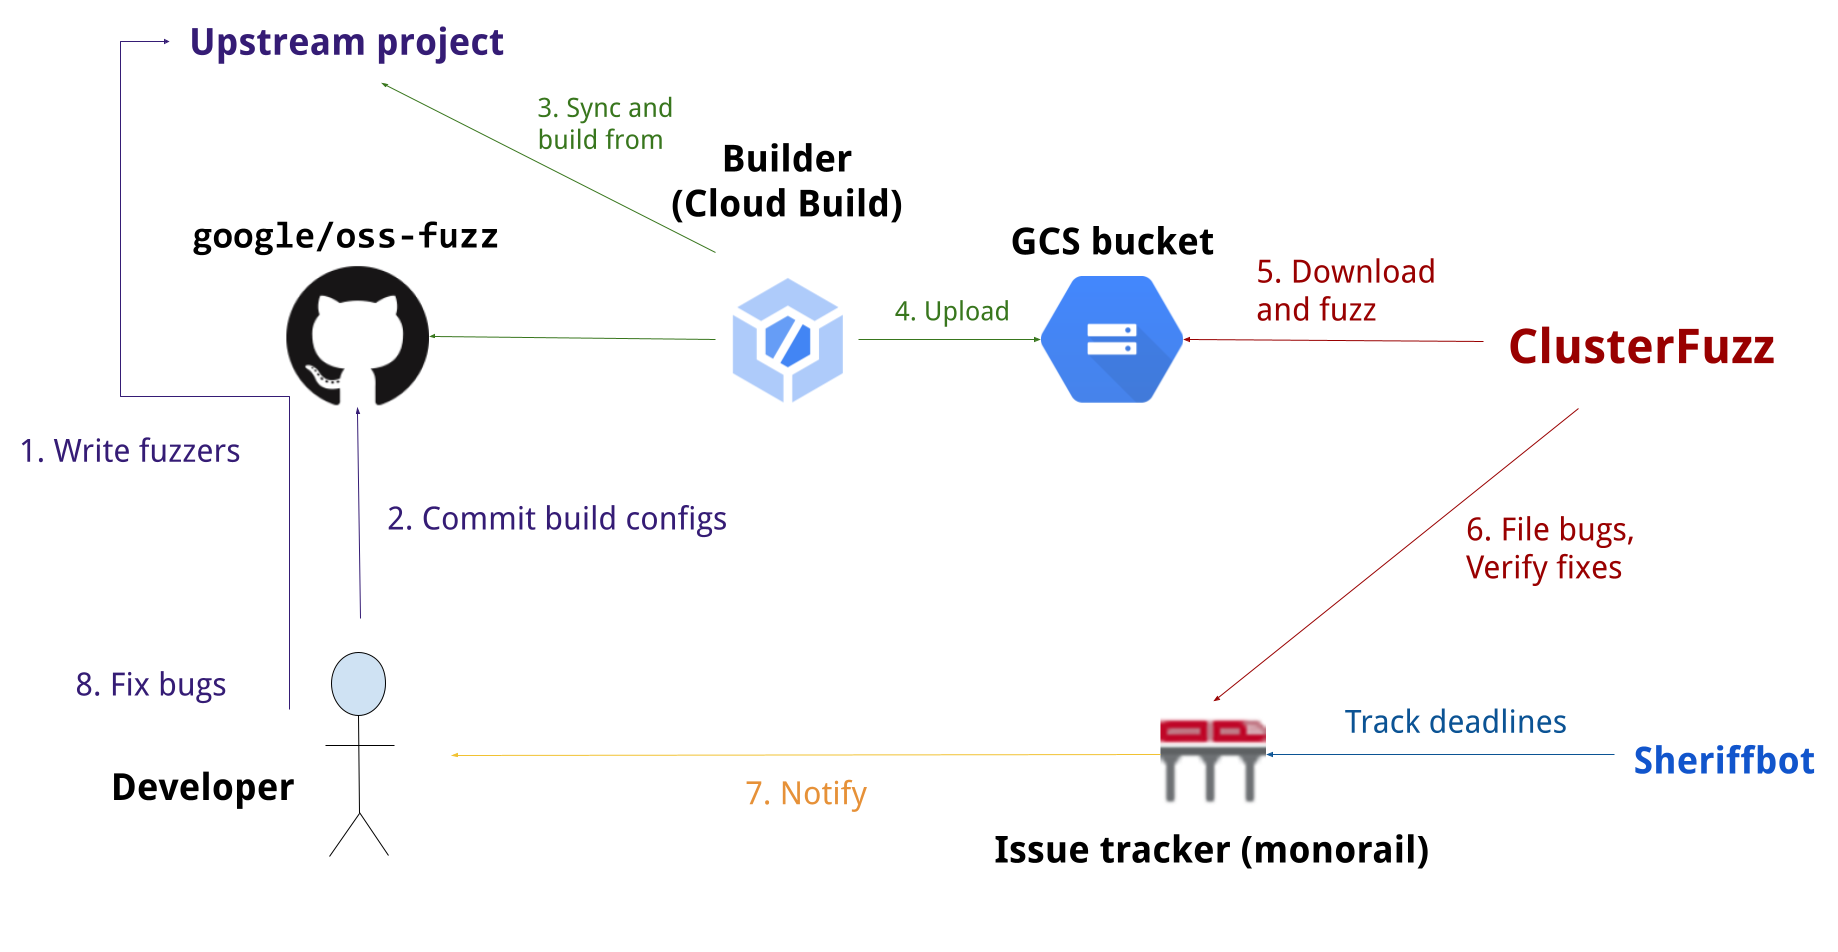
\includegraphics[width=0.65\paperwidth]{foto/oss-fuzz_architecture.png}}
\caption{OSS-Fuzz main architecture visualized \cite{ossfuzz_docs}}
\label{fig:ossfuzz_architecture}
\end{figure}

The workflow is as follows. First, the maintainers of an open-source project create one or more "fuzz targets" that are integrated into the project's build and test system \cite{libfuzzer_docs}, where a "fuzz target" defines a function that takes an input (in this thesis, an array of bytes) and performs some operations on said to test a specific API or program's functionality. Developers are also expected to provide up-to-date corpus seeds, which will be used by the chosen fuzzers for cross-mutations and improve the fuzz target’s coverage. All these resources, along with instructions on how to build and fuzz the targets, are uploaded to a Google Cloud Service Bucket, a file-hosting service acting as a middle point between OSS-Fuzz and its fuzzing back-end ClusterFuzz.

Then, a project's fuzzing session lasts (at most) 6 hours, evenly distributed across all fuzz targets with a minimum of 10 minutes per fuzz target, and \textit{ensemble fuzzing} is used when binaries are configured for multiple fuzzing engines (see figure \ref{fig:continuous_fuzzing}). Both the corpora used as input to the tests and the corpora produced as results of a successful fuzzing session (both also called \textit{queues}) are publicly available and stored in the project's Google Cloud for research purposes and \textit{regression testing}, i.e. testing a program against old inputs to ensure that previously tested functionality still works as intended and that fixed bugs do not reappear.

Finally, any bug discovered is reported to the OSS-Fuzz issue tracker \cite{ossfuzz_bugtracker}, which uses the metadata sent by ClusterFuzz to create its report. Developers have 3 ways of dealing with this situation: they can commit new changes to fix the bug (verified by ClusterFuzz before closing an issue), assign the tag "WontFix" to the bug and notify that it will not be solved, or simply ignore it altogether. 



\newpage
To be accepted by OSS-Fuzz, a project must be relevant and/or critical to the global IT infrastructure and it must have a significant user base: to check if your project is eligible, Google provides a mathematical formula to calculate its "Open-Source Project Criticality Score" \cite{score} in a range between 0 \textit{(least critical)} and 1 \textit{(most critical)}, where $\alpha_i$ refers to the "weight" of an indicator and $T_i$ to its maximum allowed value:

\begin{equation}
    CriticalityScore = \frac{1}{\sum \alpha_i}\  \sum_i \alpha_i \ \frac{\log(1+S_i)}{\log(1+\max(S_i,T_i))}
\end{equation}
\ \\
The parameters evaluated are the following:
\begin{itemize}
    \item \textbf{created-since} ($\alpha_i = 1$, $T_i = 120$): months since the project was created, older projects have a higher chance of being widely used or dependent on
    \item \textbf{updated-since} ($\alpha_i = -1$, $T_i = 120$): months since the project's last update, unmaintained projects with no recent commits have a higher chance of being less relied upon
    \item \textbf{contributor-count} ($\alpha_i = 2$, $T_i = 5000$): number of commits made by project contributors, involvement of different contributors indicates a project importance
    \item \textbf{org-count} ($\alpha_i = 1$, $T_i = 10$): number of distinct organizations contributing to the project, indicates cross-organization dependency
    \item \textbf{commit-frequency} ($\alpha_i = 1$, $T_i = 1000$): average number of commits per week over the last year, code that is constantly changing may be more susceptible to vulnerabilities
    \item \textbf{recent-releases-count} ($\alpha_i = 0.5$, $T_i = 26$): number of releases in the last year, frequent releases indicate user dependency
    \item \textbf{closed-issues-count} ($\alpha_i = 0.5$, $T_i = 5000$): number of issues closed in the last 90 days, indicates contributor involvement and focus on resolving user issues
    \item \textbf{updated-issues-count} ($\alpha_i = 0.5$, $T_i = 5000$): number of issues updated in the last 90 days, indicates high contributor involvement
    \item \textbf{comment-frequency} ($\alpha_i = 1$, $T_i = 15$): average number of comments per issue in the last 90 days, indicates user activity and dependence
    \item \textbf{dependents-count} ($\alpha_i = 2$, $T_i = 500000$): number of project mentions in the commit messages, indicates repository use
\end{itemize}
\ \\
Only projects scoring a value $\geq 0.7$ may be eligible to be integrated in the OSS-Fuzz campaign.


\newpage
Assuming your project satisfies the score requirements, developers issue a "pull request" on the OSS-Fuzz repository providing the following 3 files, which are periodically checked and validated by a bot before accepting/rejecting them.

\paragraph{project.yaml} Configuration file that contains metadata regarding who owns the project, how to contact them when filing bug reports, and configuration parameters about the fuzzing sessions, needed by OSS-Fuzz to correctly provide its services.
Some of the most common information reported are:
\begin{itemize}
    \item \textbf{homepage:} URL to the project homepage
    \item \textbf{language:} programming language used to write the project (C, C++, Go, Rust, Python, JVM languages, Swift)
    \item \textbf{primary\_contacts:} list of email addresses that are automatically CC'd on crash reports and fuzzer statistics
    \item \textbf{main\_repo:} path to the source repository where the project is hosted
    \item \textbf{vendor\_ccs:} \textit{optional}, list of email addresses of vendors who want access to bug reports
    \item \textbf{sanitizers:} \textit{optional}, list of sanitizers available in the project (address, undefined, memory)
    \item \textbf{architectures:} \textit{optional}, list of architectures that can build the project (supported only x86\_64 and i386)
    \item \textbf{fuzzing\_engines:} \textit{optional}, list of available fuzzing engines (libfuzzer, afl, honggfuzz and centipede), if not specified "libfuzzer" is used
    \item \textbf{builds\_per\_day:} \textit{optional}, number of times a project should be built per day, OSS-Fuzz allows up to 4 builds per day and builds once per day by default
\end{itemize}

\paragraph{Dockerfile} To avoid having developers create and maintain their own customized Docker containers and create a homogeneous and standard environment, OSS-Fuzz provides several "base images" based on Ubuntu 20.04 for each supported language containing the most common compilers and toolchains needed to build the project, along with some customized terminal commands useful to prepare the testing environment provided. Each project builds its own testing environment starting from the most appropriate base image, runs a series of "apt-get" and "git clone" commands to download and install all the necessary packages and dependencies, and finally pulls all the resources and fuzz targets from the project repository.

\paragraph{build.sh} Script that runs inside the Docker container defined above and performs all the operations required to build the project and the fuzzing targets to be tested. To provide a more flexible and accessible build system, all base images are configured with several environment variables regarding directory locations, compilers, and compilation flags, allowing developers to easily re-target scripts with little effort.


\newpage
To conclude, OSS-Fuzz follows a strict \textit{bug disclosure policy} \cite{bug_disclosure}.
When a bug is discovered (assuming it is not already known or a duplicate), an automatic email is generated and sent to all email addresses specified in the "project.yaml" file, and an issue is opened in the issue tracker. This email contains the report generated by ClusterFuzz, as well as an estimate of the priority and severity of the bug discovered. From this moment, the issue will be publicly visible in 90 days or after the fix is released (whichever comes earlier), meaning that anyone will have access to the causing input as well as any other debugging information related to what happened and how to reproduce the bug. Before the deadline expires, developers may request a 14-day grace period if the patch is scheduled to be released on a specific day within this extended period, in which case the public disclosure will be delayed. In all cases, Google reserves the right to move deadlines forward or backward depending on the circumstances and severity of the findings.




\subsection{FuzzBench}
The \textit{FuzzBench Project} \cite{fuzzbench_paper} is a free service that provides fuzzer developers with several real-world benchmarks tested at the Google scale, compares the results with other famous fuzzers (such as AFL and LibFuzzer), and allows them to evaluate their performance thanks to daily reports for further improvement \cite{fuzzbench_docs}.

\begin{figure}[h]
\makebox[\textwidth][c]{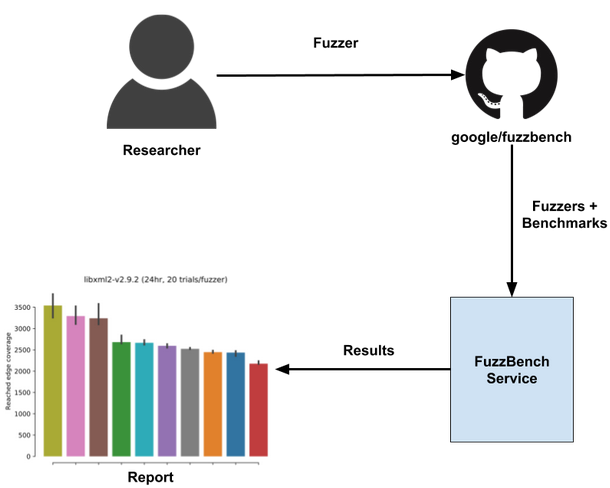
\includegraphics[width=0.7\paperwidth]{foto/fuzzbench_architecture.png}}
\caption{FuzzBench main architecture visualized \cite{fuzzbench_docs}}
\label{fig:fuzzbench_architecture}
\end{figure}

The infrastructure is structured as follows.
Initially, a fuzzer developer integrates its tool within FuzzBench using a Dockerfile, containing all the resources necessary to build targets using its fuzzer and also defining the environment where all benchmarks will be executed. Similarly to OSS-Fuzz, this process is done via "pull requests", which are automatically revisioned and accepted by bots.

Developers can then choose between two testing approaches: standard and OSS-Fuzz. In the former case, the benchmark is created by the developers themselves, which requires the definition of fuzz targets, build files, seed inputs and Docker images to correctly build, link the fuzzer to the targets and run the tests. In the latter case, the developers employ a fuzz target from a selection of OSS-Fuzz projects, maintained at a specific version known to contain bugs \cite{benchmarks} and tested using a predefined set of seed inputs: this ensures that all tests are performed using the same test environment and initial inputs across many trials, which is crucial for having a reference point when tracking a fuzzer's performance over time, while also allowing the developers to test their product on a real-world scenario. When performing fuzzing, FuzzBench also allows for coverage-oriented or bug-oriented sessions, both spanning over 24 hours with each fuzzer running 20 trials on each individual benchmark.

At the end of each day, a performance report will be created highlighting the strengths and weaknesses of the fuzzer on each benchmark, comparing individual and overall results with other integrated fuzzers both in terms of bugs found and coverage achieved.



\subsubsection{SBFT' 23} \label{conference}
FuzzBench already provides 21 open-source projects that are continuously tested by the integrated fuzzers, however preliminary analysis revealed a greater number of projects, including benchmarks not listed on the website \cite{benchmarks}. After investigating the contents of this repository and its commit history, 7 additional projects were discovered, added for only a few months and then removed to never be restored.  

These projects were added for a conference on the effectiveness of fuzzing tools called "Search-Based and Fuzzing Tools (SBFT) 2023" \cite{sbft23}, where a tool competition was created using FuzzBench as the benchmarking tool: the idea was to allow developers to integrate their fuzzers into FuzzBench, run experiments locally on a provided sample benchmark to familiarize with real open-source projects and state-of-the-art fuzzers, and analyze the provided evaluation reports to visualize the effectiveness of their products. In particular, these 7 projects were used only during the final stages of the competition, ensuring that all participants performed the final evaluations on previously untested benchmarks.

The goal of this conference was to provide a way for developers to approach continuous fuzzing frameworks, contribute to the development of FuzzBench by integrating new and effective fuzzers, and provide real-world scenarios for developers to test their tools.


\chapter{Methodology} \label{chap_3}
\ \\
The objective of this thesis was to see if there were any overlooked bugs in common fuzzing benchmarks, choosing OSS-Fuzz and FuzzBench as they are among the most popular ones. This, in turn, meant analyzing the effectiveness of such automated testing campaigns and verify how efficiently they were being employed by open-source developers.
\newline \newline
What does it mean for a bug to be "overlooked" in this context? 
\newline \newline
If we think about OSS-Fuzz, where fuzzing is performed automatically by VMs, it means to look for cases where machines failed: this could happen either due to a fault in the automation process or due to the integration choices made by the developers.
\newline
In the first case, we may talk about limits imposed by OSS-Fuzz on its resources, like tests that cause out-of-memory scenarios, timeouts or even bugs that cannot be reliably and consistently reproduced. 
In the second case, it is strictly related to the content of the \textit{project.yaml} configuration file: different sanitizers look for different types of bugs, while each fuzzing engine uses its own set of strategies to test a program, producing results that may be completely different from the other provided fuzzers.
\newline
For this reason, I focused on the latest public "fuzzing queue" made available by the developers, i.e. the corpus of inputs used by OSS-Fuzz when performing the tests.
\newline \newline
If we think about FuzzBench, where projects are actively tested by several different fuzzers, it means to look for bugs discovered in older versions that were not tested on newer ones, which obviously is a human error.
\newline
A small selection of projects from OSS-Fuzz are tested continuously by several different fuzzers, producing daily reports available both to the fuzzers and the chosen projects developers, along with public access to the corpora used to perform the tests as well as the results and the crashes found (if any). It is then responsibility of the project developers to analyze and fix these bugs, although this does not always happen.
\newline
For this reason, I focused on analyzing a chosen set of experiments between 2020 and 2024, downloading all the available crashes and testing them on latest version, hoping to find old bugs that have yet to be fixed.
\newline \newline
As previously mentioned, all relevant bugs were then appropriately reported to their respective developers.






\newpage
\section{Setting up the environment}

\matteo{Nice, we need this info. Maybe we should shift it at the end of "methodology", or at the start of "results", see which seems better} \ziosaba{I think that putting it at the beginning of "methodology" might be better, as most of the tools introduced here will be mentioned in the next sections}

All tests were performed on two separate machines, both equipped with personal installations of Ubuntu 22.04 LTS, already run-in and used.
\newline \newline \newline
Regarding tools for general purpose, I used Docker, Valgrind, Python 3, gsutil and Google Chrome.
\newline \newline
The \textit{Docker} \cite{Docker} application run the different containers needed by OSS-Fuzz to build the environment where projects will be built and tested.
\newline \newline
\textit{Valgrind} \cite{Valgrind_1}\cite{Valgrind_2} is a dynamic binary instrumentation (DBI) framework to perform analysis, profiling and management of a program during its execution.
More specifically, it was used to perform memory analysis when projects were built without sanitizers.
\newline \newline
The \textit{Python 3} language was used to create several scripts that I used to perform information scraping, reports analysis and bug deduplication.
It is also used by OSS-Fuzz to provide some functionalities, and this will be discussed later. 
\newline \newline
The \textit{gsutil} suite is a command-line tool provided by Google to access resources stored on Google Cloud Service from your local machine, and it was used to analyze the FuzzBench benchmarks and download other resources.
\newline \newline
Finally, \textit{Google Chrome} and its "development driver" were needed during the information scraping phase of this work, discussed in section \ref{selection}.
\newline \newline \newline
Regarding \textit{OSS-Fuzz}, most of the work was done on its GitHub repository, which I cloned locally on both machines.
\newline
To provide its services, OSS-Fuzz uses several python scripts that can be invoked via command-line using appropriate arguments. These commands can be used to update the projects' files and projects' images, build the project's image and its fuzzers but also download resources like corpora. 
\newline \newline \newline
Regarding \textit{FuzzBench}, most of the work was done on its Google Cloud bucket, specifically on the section where all experiments results are collected.
\newline
To access and later download the resources needed, I incorporated the \textit{gsutil} suite in a python script to perform web scraping.



\newpage
\section{OSS-Fuzz}
\subsection{Selecting the projects} \label{selection}
At the moment of writing, the OSS-Fuzz campaign includes over 1000 projects that are actively fuzzed and tested, but it would obviously be impossible to rebuild and test all of them locally also due to the language heterogeneity of such projects.
\newline
For this reason, this work focused solely on projects using the C/C++ language.
\newline
Then, to further narrow down the analysis, I identified 5 different categories of projects using the number of sanitizers used by the developers, keeping ASan as the reference due to its popularity and efficiency.
\newline
Finally, I ordered each set by "highest number of bugs issued" using the OSS-Fuzz bug tracker and tested these lists top-down until I had 5 projects for each category that were building and fuzzing correctly.
\ \\ \newline \newline
First step in this process was to extract the list of all projects written in C/C++, and this was done by performing a preliminary analysis of the \textit{project.yaml} configuration file present inside each project's directory.
\newline
\begin{figure}[h]
\centering
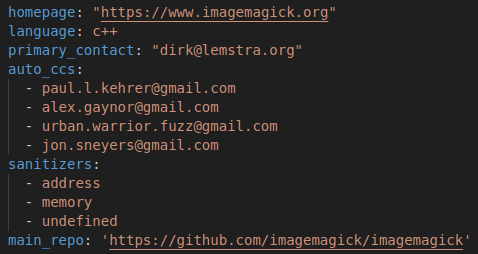
\includegraphics[scale=0.65]{foto/project_yaml.png}
\caption{Example of content from a project.yaml}
\label{fig:project_yaml}
\end{figure}
\ \\
To retrieve the language used by each project, I initially wrote a simple Python script taking as input the OSS-Fuzz "project" directory.
\newline
Then, the script opened the directory list of the argument provided and iteratively explored each project's directory looking for the aforementioned configuration file: assuming the file was found, it then opened the file and scanned each line looking for the "language: c" string, eventually saving the name of such projects in a list.
\newline \newline
This yielded a total of 524 projects out of 1277 written using C/C++.


\newpage
To perform the categorization of the projects depending on the number of sanitizers used, I extended the previous script to also look for the strings "address", "memory" and "undefined", shown on image \ref{fig:project_yaml}.
\newline
The assignment uses a binary logic on decimal values, starting each project from 0 and giving each sanitizer a different value (1, 10, 100), so that by summing them I could easily understand which sanitizers were found in its configuration file.
\newline \newline
Out of the previous 524 projects, the results were as follows: 238 used all sanitizers, 22 used ASan and MSan, 62 used ASan and UBSan, 46 used only ASan and 156 did not use any sanitizers.
\ \\ \newline \newline
The next step was retrieving the number of discovered bugs of each project, and this required a thorough analysis of the "OSS-Fuzz Issue Tracker" website. \cite{ossfuzz_bugtracker}
\newline
\begin{figure}[h]
\makebox[\textwidth][c]{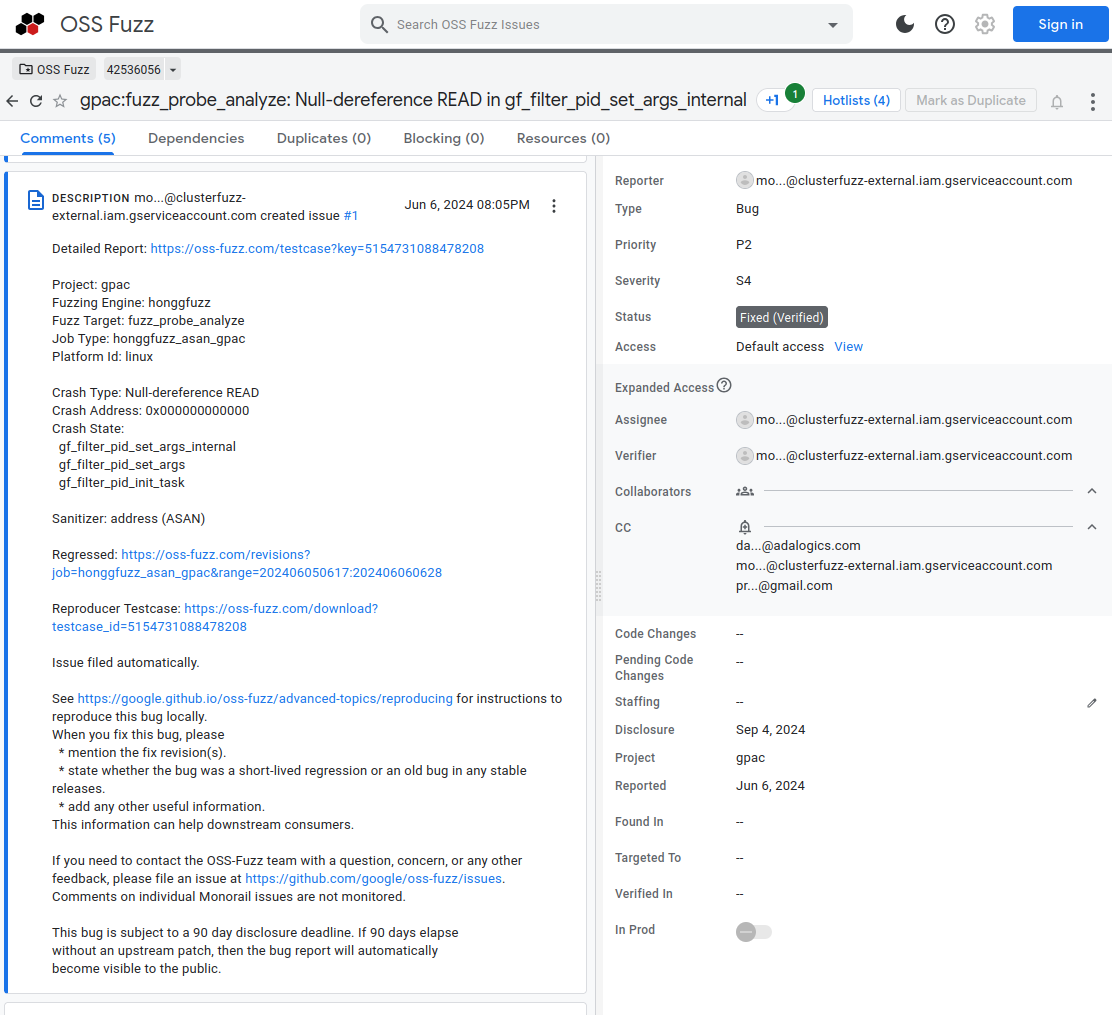
\includegraphics[width=0.69\paperwidth]{foto/issue.png}}
\caption{Example of bug report \cite{ossfuzz_bugtracker}}
\label{fig:issue}
\end{figure}
\ \\
At the moment of writing, the issue tracker platform was changed from "Monorail" to "Google Sites", so most of the work described here may no longer work as intended.




\newpage
Given that Monorail APIs could only be used by projects' developers registered to OSS-Fuzz and that there weren't any files that could be used for an offline analysis, I had to perform website scraping on the individual issues to retrieve the information. 
\newline
To do this, I used as reference a GitHub repository written by Zhen Yu Ding called "Monorail Scraper" \cite{scraper}, a tool to scrape and retrieve data from Monorail, that also included functionalities for ClusterFuzz-generated OSS-Fuzz issues.
\newline \newline
The tool relies on the Google Chrome web browser and their testing development tool called "ChromeDriver" \cite{driver}: this is an autonomous web server implementing "W3C WebDriver" \cite{driver_standard}, a standard providing a remote interface to control user-agents and a set of interfaces to perform analysis and manipulation of DOM elements.
\newline
Essentially, this allows the user to write scripts that, in turn, instruct the Google Chrome browser to visit a specific web page and possibly performs some interaction with it, like pushing a button, compiling a form or visiting another webpage by exploring the DOM elements.  
\newline \newline
In this work, I focused on the functionalities for the analysis of OSS-Fuzz reports.
\newline
Initially, the user provides a range of "report IDs" to retrieve.
\newline
Then, the tool opens a new Google Chrome instance and performs a connection to a specific link in the Monorail website, attempting the reconnection only once if the first one fails. If the resulting DOM shows a login form, it means that the requested bug is still in the disclosure window, in which case the next ID is analyzed.
\newline
Assuming that the requested report is publicly accessible, the DOM is scanned for key information.
During this phase, given that the project is already few years old, I had to make some minor corrections and adjustments as some parameters collected were changed and/or missing altogether.
\newline
All the information collected by each report was then stored in JSON files.
\newline
\begin{figure}[h]
\makebox[\textwidth][c]{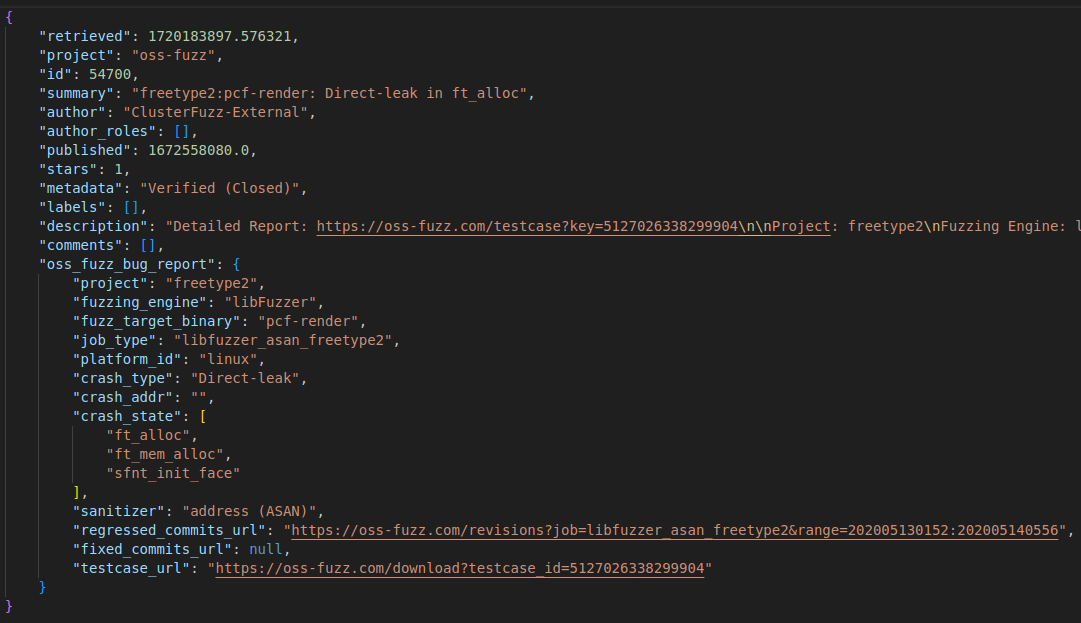
\includegraphics[width=0.66\paperwidth]{foto/json.png}}
\caption{Example of information collected from reports in JSON}
\label{fig:report}
\end{figure}
\ \\
The analysis was performed on all bugs between 2023-01-01 and 2024-06-31, for a total of 11743 collected reports.



\newpage
The second to last step was to analyze the previously obtained JSON files and make a list of the most bugged projects for each category.
\newline
To do this, I initially wrote a simple Python script that takes as input the JSON files and analyzes the information fields collected.
\newline
First, I checked the \textit{"metadata"} field for values like "WontFix", "Duplicate" or "Invalid": the first means that the developers themselves tagged that specific bug as non-relevant and will not be addressed in the future, the second refers to a report for a bug that has been already issued but triggered by a different testcase, while the last one means that the reported bug could not be reliably reproduced.
\newline
Then, I checked the \textit{"description"} field for manual reports, as they were not meaningful towards the final results. 
\newline
Assuming the report analyzed is valid and generated by ClusterFuzz, I retrieved the project name from the \textit{"oss\_fuzz\_bug\_report"} fields and used a dictionary key-value to keep track of the number of bugs reported for each project. 
\newline
\begin{figure}[h]
\centering
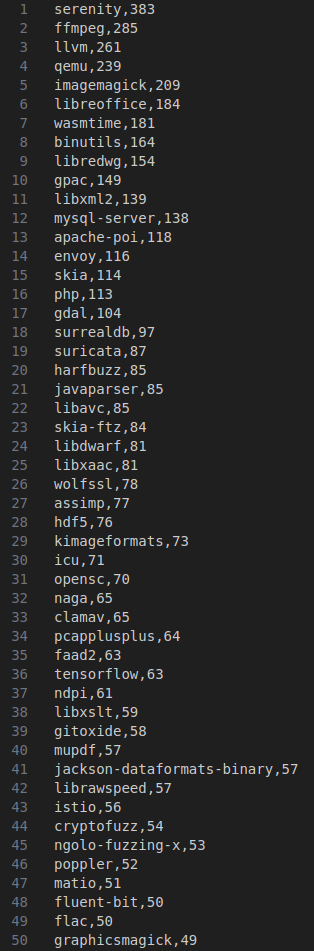
\includegraphics[scale=0.44]{foto/list.png}
\caption{Excerpt of the 50 most bugged projects}
\label{fig:list}
\end{figure}

\newpage
The last step was to analyze each project individually and determine which harness produced the highest number of reports.
\newline
Given the previous script, I extended it to take as input also a project name, so that the parsing of the JSON file focused only on reports for that particular project, and the dictionary key-value was now used to keep track of the number of bugs produced by each fuzzing target binary.
\ \\ \newline \newline
All this resulted in the following projects and harnesses being tested:
\begin{itemize}
  \item \textbf{All Sanitizers}
  \begin{itemize}
    \item binutils (fuzz\_objdump\_safe)
    \item harfbuzz (hb-subset-fuzzer)
    \item imagemagick (encoder\_heic\_fuzzer)
    \item libxml2 (valid)
    \item skia (skruntimeeffect)
  \end{itemize}
  \item \textbf{ASan + MSan}
  \begin{itemize}
    \item ghostscript (gs\_device\_pdfwrite\_fuzzer)
    \item libyang (lyd\_parse\_mem\_json)
    \item wasmedge (wasmedge-fuzztool)
    \item openjpeg (opj\_decompress\_fuzz\_J2K)
    \item myanmar-tools (zawgyi\_detector\_fuzz\_target)
  \end{itemize}
  \item \textbf{ASan + UBSan}
  \begin{itemize}
    \item cairo (svg-render-fuzzer)
    \item clamav (clamav\_dbload\_YARA\_fuzzer)
    \item freerdp (TestFuzzCoreClient)
    \item tarantool (luaL\_loadbuffer\_fuzzer)
    \item vlc (vlc-demux-dec-libfuzzer)
  \end{itemize}
  \item \textbf{ASan only}
  \begin{itemize}
    \item fwupd (uswid\_fuzzer)
    \item glslang (compile\_fuzzer)
    \item inchi (inchi\_input\_fuzzer)
    \item radare2 (ia\_fuzz)
    \item zeek (zeek-ftp-fuzzer)
  \end{itemize}
  \item \textbf{No Sanitizers}
  \begin{itemize}
    \item fluent-bit (flb-it-fuzz-cmetric\_decode\_fuzz\_OSSFUZZ)
    \item gpac (fuzz\_probe\_analyze)
    \item libdwarf (fuzz\_debug\_str)
    \item libredwg (llvmfuzz)
    \item serenity (FuzzJs)
  \end{itemize}
\end{itemize}








\newpage
\subsection{Testing with OSS-Fuzz}
The OSS-Fuzz repository contains several tools to build and test the available projects, as well as debugging and reproduction scripts.
\newline
Most of the tools used in this work are provided by the "helper.py" script, which I used to download a project's Docker image, build the fuzzers and download the public corpora made available by the developers.
\newline \newline
The commands used are:
\begin{verbatim}
    $ python3 helper.py pull_images 

    $ python3 helper.py build_image {project_name}

    $ python3 helper.py build_fuzzers {project_name}
        --sanitizer={address(default),memory,undefined,none} 
            --engine={libfuzzer(default),afl, honggfuzz, centipede}
        
    $ python3 helper.py download_corpora 
        --project={project_name} --fuzz-target={harness_name}
\end{verbatim}
\ \\
The \verb|pull_images| argument connects to OSS-Fuzz's Google Bucket to download and update all the Docker "base images" on your local machine, which are used by all projects as the base image to create their respective testing environment.
\newline \newline
The \verb|build_image| argument takes as input the name of a project and builds its Dockerfile, creating a new image on your local machine that will be later used to perform fuzzing. During this process, all dependencies and resources needed to correctly compile the fuzzers are downloaded and installed, including the main \textit{build.sh} script. It was used in conjunction with daily \verb|git pull| on the OSS-Fuzz repository, to make sure that I was always building the latest version. 
\newline \newline
The \verb|build_fuzzers| argument takes as input the name of a project and a list of possible sanitizers and fuzzing engines to be used during the compilation of the fuzz targets. Although this command accepts only one sanitizer at a time, it's possible to mix them by acting on some environment variables provided by the base images. Finally, this script acts as a "wrapper" for a much more complex Docker command, that creates the project's Docker image using some specific environment variables and invokes the execution of the \textit{build.sh} script.
\newline \newline
The \verb|download_corpora| argument takes as input a project name and a fuzz target, it then connects to the project's Google Bucket and downloads the latest public corpus for the provided fuzz target.
\newline \newline \newline
After executing these commands, three new directories are created.
\newline
The \verb|out| directory contained the project's directory where all built files were saved, including libraries, fuzz targets and other files created by the selected fuzzer.
\newline
The \verb|work| directory acted as a temporary location to store intermediate files during the building process and the fuzzing sessions.
\newline
The \verb|corpus| directory contained the downloaded corpora stored as zip files.



\newpage
To prepare the tests, I was tasked with building the chosen harnesses using all possible values for sanitizers, meaning that each project was compiled 4 times: with ASan only, with MSan only, with UBSan only and without any sanitizer.
\newline
Moreover, all projects were built using AFL as fuzzing engine, as it is the current state-of-the-art fuzzer. 
\newline \newline
The tests were performed inside each project's Docker image, created and configured using the following command:
\begin{verbatim}
    $ docker run --rm --privileged --platform linux/amd64 
        -v /oss-fuzz/build/out/{project_name}/:/out/
        -v /oss-fuzz/build/corpus/{project_name}/:/corpus/    
        -v /home/zio-saba/Scrivania/TESI/logfiles/:/logfiles/ 
        -it  gcr.io/oss-fuzz/{project_name} /bin/bash
\end{verbatim}
\ \\
This is a shorter and modified version of the command invoked by the \verb|build_fuzzer| wrapper.
\newline \newline
The first few parameters are needed to create a privileged instance of Docker and specify the running platform on which the fuzz targets will be tested.
\newline \newline
The arguments starting with \verb|-v| are used to create a shared directory in the Docker container, which means linking a local directory to a virtual one created inside the container. This was needed to make sure that I could access the resources stored locally on my machine (i.e. fuzz targets, libraries and their corpus) from inside the Docker container used for the tests.
\newline \newline
The last line invokes the project image to load as well as making it interactive by spawning a \verb|/bin/bash| process.
\newline \newline \newline \newline
Once the Docker images has been loaded and ready to use, some final adjustments were performed to perform the tests.
\newline \newline
All tests performed on fuzz targets built with MSan required the sanitizer's libraries to be copied in some specific locations, using the following commands:
\begin{verbatim}
    $ cp -R /usr/msan/lib/* /usr/local/lib/x86_64-unknown-linux-gnu/
    $ cp -R /usr/msan/include/* /usr/local/include
\end{verbatim}
\ \\
All tests performed on fuzz targets built without sanitizers relied on Valgrind to perform binary analysis and profiling, installed using the following command:\begin{verbatim}
    $ sudo apt install gdb valgrind
\end{verbatim}
\ \\
Sometimes, the \verb|apt| tool was not available in a specific Docker container: this is because all base images provided by OSS-Fuzz contain a minimal installation of Linux Ubuntu with only some key packages that are usually enough to compile a programs, such as compiler, assembler, text editors and standard libraries.
\newline
In such cases, the \verb|unminimize| command was executed, which essentially "unpacks" the container and reverts it to a standard Ubuntu image, reinstalling all the default packages as well as standard additional tools.



\newpage
When testing fuzz targets built with ASan, MSan or UBSan, I used the following command:
\begin{verbatim}
    $ for i in /corpus/*; do 
        echo "TEST" $i; 
        echo "TEST" $i >> /logfiles/PROJECT_SANITIZER-NAME.log; 
        ./{fuzz_target} $i &>> /logfiles/PROJECT_SANITIZER-NAME.log; 
      done
\end{verbatim}
\ \\
This commands uses the shell \verb|for| construct to scan all files found in the "corpus" directory.
\newline
Then, it prints the name of the current testcase on the terminal, which I used for monitoring purposes.
\newline
Finally, it prints the name of the current testcase and the results of the fuzz target executed on that particular testcase on a log file.
\newline
\begin{figure}[h]
\makebox[\textwidth][c]{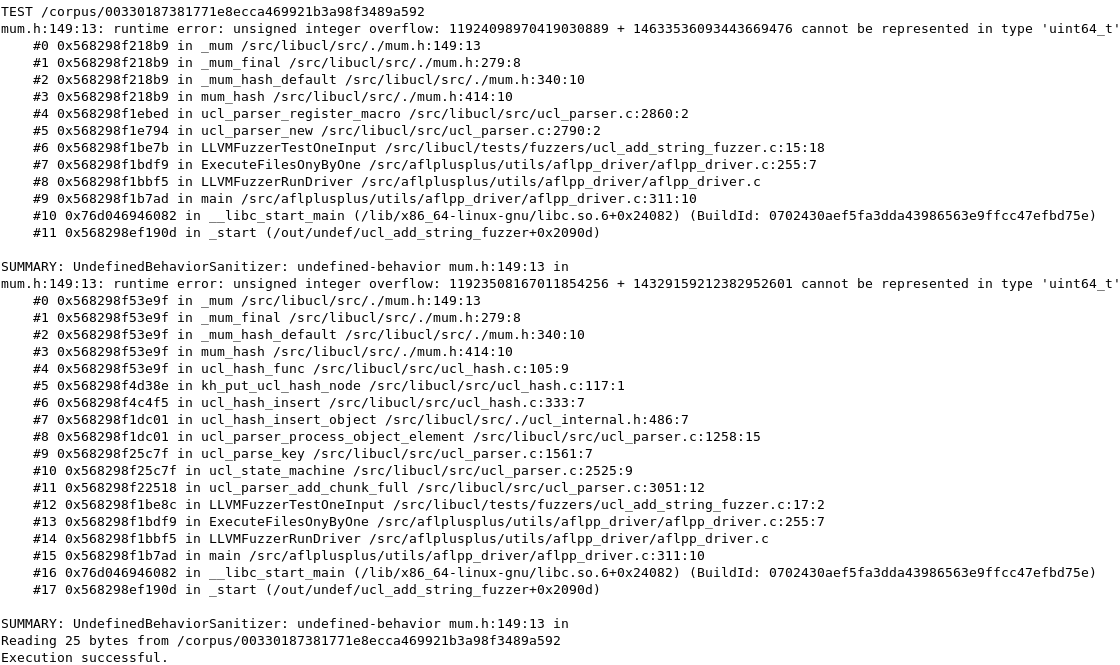
\includegraphics[width=0.8\paperwidth]{foto/ubsan_example.png}}
\caption{Example of integer-overflow bug reported by UBSan}
\label{fig:ubsan_example}
\end{figure}
\ \\



\newpage
When testing fuzz targets built without any sanitizers, I used Valgrind to analyze and profile the binary's execution, using the following command:
\begin{verbatim}
    $ for i in /corpus/*; do 
        echo "TEST" $i; 
        valgrind --log-fd=9 9>>/logfiles/PROJECT_valgrind.log 
            ./{fuzz_target} $i >> /logfiles/PROJECT_valgrind.log 
            && echo -e "\n\n" >> /logfiles/PROJECT_valgrind.log; 
      done
\end{verbatim}
\ \\
Again, I used the shell \verb|for| construct to scan all files found in the "corpus" directory and print the name of the current testcase on the terminal for monitoring purposes.
\newline
Then, I invoked Valgrind with a custom file descriptor, which allowed me to capture \verb|STDERR| and print it in the log file.
\newline
Finally, it prints the result of the fuzz target executed on that particular testcase on a log file.
\newline
\begin{figure}[h]
\makebox[\textwidth][c]{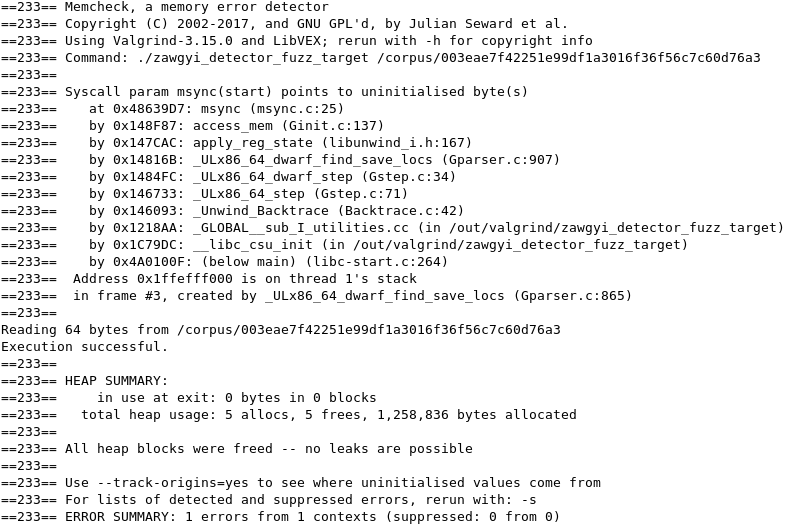
\includegraphics[width=0.65\paperwidth]{foto/valgrind_example.png}}
\caption{Example of use-of-uninitialized-memory (UUM) bug reported by Valgrind}
\label{fig:valgrind_example}
\end{figure}
\ \\




\newpage
However, not all projects built on their first attempt.
\newline \newline
In most cases, the building process failed due to missing libraries: for example, libraries like \verb|pthread| and \verb|math| were often automatically added by the sanitizers.
\newline
Other times, libraries were not being correctly linked and/or were missing crucial compiling flags, like \verb|-ldl| and \verb|-lz|.
\newline \newline
To fix these problems, I had to manually modify the source files and compile the fuzz targets from inside the Docker container, using a command similar to the one executed by \verb|compile_fuzzers|:
\begin{verbatim}
    $ docker run --rm --privileged --platform linux/amd64 
        -e PROJECT_NAME={project_name} -e HELPER=True 
        -e FUZZING_LANGUAGE=c++ 
        -e FUZZING_ENGINE=afl 
        -e SANITIZER={address,memory,undefined,none} 
        -v /oss-fuzz/build/out/{project_name}/:/out/   
        -v /oss-fuzz/build/work/{project_name}/:/work/
        -it  gcr.io/oss-fuzz/{project_name} /bin/bash
\end{verbatim}
\ \\
Similarly to before, the first few parameters are needed to create a privileged instance of Docker and specify the running platform on which the fuzz targets will be tested, the arguments starting with \verb|-v| are used to create a shared directory in the Docker container and the last line invokes the project image to load as well as making it interactive by spawning a \verb|/bin/bash| process.
\newline \newline
The novelty lies in the arguments starting with \verb|-e|, which can be used to override the environment variables provided by the Docker image.
\newline
These variables can be used by the source files to compile a program using the most appropriate compile flags, fuzzing engine and sanitizers, and they can be easily modified by the user when creating the Docker image to easily re-target the compilation with little to none effort.
\newline \newline
After loading the Docker image and modifying the source files, the command \verb|compile| invokes the execution of the "build.sh" script and starts the building process for the fuzz targets.



\newpage
\section{FuzzBench}
\subsection{Selecting the projects}
The FuzzBench campaign started in 2020, performing tests almost daily for the past 4 years, providing valuable information to both fuzzers developers and the developers of the selected projects that have been integrated as benchmarks.
\newline \newline
The FuzzBench data is structured as follow:
\begin{figure}[h]
\centering
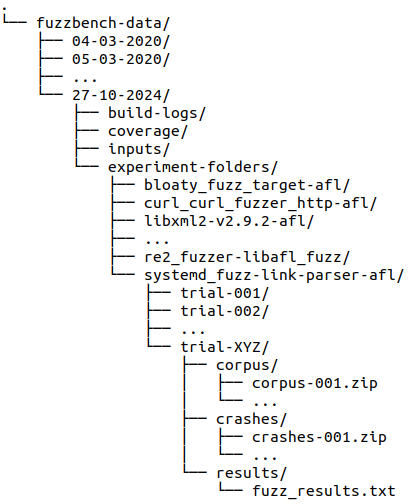
\includegraphics[scale=0.4]{foto/tree.png}
\caption{FuzzBench's Google Cloud directory tree}
\label{fig:tree}
\end{figure}
\ \\
All data is grouped by test date.
\newline \newline
Each test set is composed by several key information.
\newline 
The \verb|build-logs| folders contains the logs generated by the fuzzers when building the fuzz targets.
\newline 
The \verb|coverage| folder contains information related to the coverage achieved by each fuzzer on the different projects tested that day
\newline
The \verb|input| folder contains the binaries executed to compile the different fuzz targets.
\newline
The \verb|experiment-folders| folder contains all the data related to the testing session.
\newline \newline
Following the experiments, each project has its own folder that specifies the name of the project, the fuzz target tested, the fuzzing engine used and sometimes also the objective of the session (bugs, coverage, correctness). 
\newline
Then, each project undergoes several fuzzing sessions, identified by \verb|trial| folders.
\newline \newline
Finally, each trial provides the information relevant to this work.
\newline
The \verb|corpus| folder contains several corpora stored as zip files.
\newline
The \verb|crashes| folder contains all the crashes found in each trial as a separate zip file.
\newline
The \verb|results| folder contains the cumulative log of all fuzzing sessions.
\newline \newline
The objective of this analysis was to download the content of the \verb|crashes| directories of several experiments, build the latest version of the respective projects and verify whether all these old crashes have been fixed or not.


\newpage
Considering that downloading and analyzing the content of potentially tens of millions zip files would require several month, I was tasked with finding a way to differentiate between the different types of test sessions.
\newline \newline
To do this, I found the \textit{experiment-requests.yaml} configuration file \cite{exp_yaml} inside the FuzzBench repository, which contained
all information related to the type of tests conducted, the projects tested as well as all the fuzzing engines used:
\newline
\begin{figure}[h]
\centering
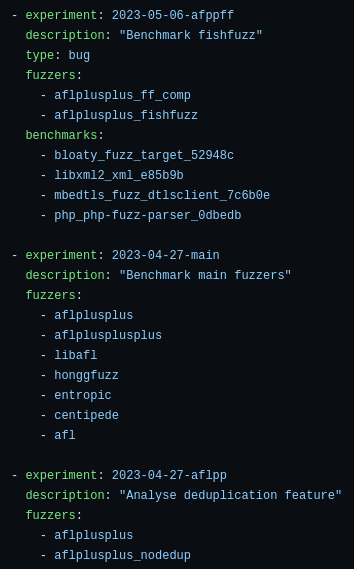
\includegraphics[scale=0.55]{foto/exp_yaml.png}
\caption{Excerpt fron the experiment configuration file}
\label{fig:exp_yaml}
\end{figure}
\ \\
Then, similarly to the process followed in section \ref{selection}, I wrote a simple Python script taking as input the above file and storing the name of all those experiments containing the string "type: bug".
\newline \newline
However, this file only contained information on all experiments between 2020 and 2023, and unfortunately I was not able to find any reference on all the experiments performed in 2024, forcing me to analyze all of them.



\newpage
Then, I was tasked with selecting the projects that will be analyzed.
\newline
Fuzzbench already provides a comprehensive list of open-source projects that have been integrated and continuously tested \cite{benchmarks}, however preliminary analysis on its Google Cloud Bucket (GCB) yielded a greater number of projects not listed on their website.
\newline
After investigating the content of its repository and GCB, I discovered 7 additional projects that were added to the GitHub repository for only few months, and later removed and never restored again. More specifically, these projects were added as part of a conference on the effectiveness of fuzzing tools called "Search-Based and Fuzzing Tools (SBFT) '23" \cite{sbft23} and provided to all researchers as the benchmarks on which they had to test their fuzzers.
\newline
It's interesting to notice that due to their relevance, these 7 projects will be later responsible for 90\% of the crash collected.
\newline \newline
Finally, to analyze all the experiments on FuzzBench GCB and download their content, I used the \textit{gsutil} suite provided by Google, which works similarly to the \verb|ls|, \verb|mv| and \verb|cp| command of the Linux shell, except that it takes as argument the url of a Gollge Cloud resource.
\newline
To retrieve all the resources needed, I wrote a Python script that essentially performs horizontal scraping over the directory tree shown in figure \ref{fig:tree}, storing at each intermediate steps the link of the next resource to list using the \verb|gsutil ls| command.
\newline \newline \newline
In conclusion, this analysis yielded 971656 zip file, for a total of (qualche milione di) crashes, and the following projects and harnesses being tested:
\newline
\noindent
\begin{tabularx}{\textwidth}{
    @{\hspace{2em}}% Space for left bullet
    >{\leavevmode\llap{\textbullet~}\raggedright\rule{0pt}{3ex}}% Left bullet + formatting of column
    X% Left column specification
    @{\quad\hspace{1em}}% Space between columns + right bullet space
    >{\leavevmode\llap{\textbullet~}\raggedright\arraybackslash}% Right bullet + formatting of column
    X% Right column specification
    @{}% No column space on right
  }
  arrow (parquet-arrow-fuzz) & aspell (aspell\_fuzzer) \\
  assimp (assimp\_fuzzer) & bloaty (fuzz\_target) \\
  curl (curl\_fuzzer\_http) & ffmpeg (ffmpeg\_demuxer\_fuzzer) \\
  file (magic\_fuzzer) & freetype2 (ftfuzzer) \\
  grok (grk\_decompress\_fuzzer) & harfbuzz (hb-shape-fuzzer) \\
  jsoncpp (jsoncpp\_fuzzer) & lcms (cms\_transform\_fuzzer) \\
  libaom (av1\_dec\_fuzzer) & libjpeg-turbo (libjpeg\_turbo\_fuzzer) \\
  libpcap (fuzz\_both) & libpng (libpng\_read\_fuzzer) \\
  libxml2 (xml) & mbedtls (fuzz\_dtlsclient) \\
  openssl (x509) & openthread (ot-ip6-send-fuzzer) \\
  php (php-fuzz-parser) & proj4 (proj\_crs\_to\_crs\_fuzzer) \\
  re2 (re2\_fuzzer) & sqlite3 (ossfuzz) \\
  systemd (fuzz-link-parser) & vorbis (decode\_fuzzer) \\
  woff2 (convert\_woff2ttf\_fuzzer) & zlib (zlib\_uncompress\_fuzzer)  
\end{tabularx}




\newpage
\subsection{Testing with FuzzBench}
Explain how projects were built....
\newline \newline
Explain how tests were automated and their duration...




\ziosaba{All the collected crashes were divided in 3 categories:
\begin{itemize}
    \item \textbf{crash:} inputs leading to any scenario that forces the system to close the process, like SEGV and heap/stack buffer overflows
    \item \textbf{out-of-memory (oom):} inputs inducing memory leaks or using huge allocation sizes to purposely test fail-safe mechanisms
    \item \textbf{timeout:} inputs that are either very long to parse or that purposely introduce unnecessary operations, again to test the resiliency of the program 
\end{itemize}}



\newpage
When i testef fuzzbench and had to build using ASan + UBSan, i Didi this:
\begin{verbatim}
    $ docker run --rm --privileged 
        --platform linux/amd64 --memory=16g 
        -e PROJECT_NAME={project_name} -e HELPER=True 
        -e FUZZING_LANGUAGE=c++ -e FUZZING_ENGINE=afl 
        -e SANITIZER=address 
        -e SANITIZER_FLAGS_address="
            -fsanitize=address,array-bounds,bool,builtin,enum,
                integer-divide-by-zero,null,object-size,return,
                returns-nonnull-attribute,shift,
                signed-integer-overflow,unsigned-integer-overflow,
                unreachable,vla-bound,vptr
            -fno-sanitize-recover=array-bounds,bool,builtin,enum,
                integer-divide-by-zero,null,object-size,return,
                returns-nonnull-attribute,shift,
                signed-integer-overflow,unreachable,
                vla-bound,vptr 
            -fsanitize-address-use-after-scope" 
        -v /oss-fuzz/build/out/{project_name}/:/out/  
        -v /oss-fuzz/build/work/{project_name}/:/work/
        -v /oss-fuzz/build/corpus/{project_name}/:/corpus/
        -v /home/zio-saba/Scrivania/TESI/logfiles/:/logfiles/  
        -it  gcr.io/oss-fuzz/{project_name} /bin/bash
\end{verbatim}



\chapter{Results} \label{chap_4}
\ \\
To correctly analyze and categorize the bugs discovered you need to perform \textit{bug deduplication}, a technique used to remove all inputs that produced the same results, which is crucial to remove unnecessary data from the results and make the bug analysis work less tedious for the developer.
\newline
There are several strategies that can be applied to deduplicate bugs, but it's important to mention that there is no fool-proof methodology that produces perfect results on all possible scenarios, and this is because which information you are using as reference and their number will (almost always) lead to partial loss of data.
\newline
Given that this work focused primarily on OSS-Fuzz, I decided to employ the same approach used by them when generating bug reports, where they use the fields "Crash Type" and "Crash state" as the main references (Figure \ref{fig:issue}).
\newline
To do this, I used several Python scripts (one for each sanitizer and one for Valgrind) that analyzed the logs generated by the fuzzing sessions, and deduplication was performed by its \textit{"error type"} and the last 3 stack entries from where the error occurred.
\newline \newline
Then, \textit{bug triage} was performed, analyzing more in depth where the bug occurred, why it happened and assigning a priority in the range "Low", "Medium" and "High". This required a manual investigation of each bug individually, statically and dynamically (when available), to have a more clear understanding of the problem and potentially provide suggestions to the developers regarding the fix.
\newline
This step was also important to refine the previous deduplication step.
\newline
Assume the situation where two inputs triggered two (apparently) different bugs because they have distinct stack flows: if the bug originated from the same function, it meant that two different execution flows triggered the same error. In this case, a common practice is to fix one of them and then use the other input as an additional check for correctness.
\newline \newline
Finally, all recorded bugs for a project, along with their log and fuzz targets were reported to their respective developers.
\newline
At the moment of writing, unfortunately, not all developers answered and/or acknowledged the reported bugs.






\newpage
\section{OSS-Fuzz (aggiornare la tabella fino all'ultimo!)}
\ \\
\begin{adjustbox}{width=\textwidth,center}
\begin{tabular}{|l|l|l|l|l|l|l|l|l|}
\hline
\textbf{Project} & \textbf{Sanitizers} & \textbf{Queue size} & \textbf{Crashes} & \textbf{ASan} & \textbf{MSan} & \textbf{UBSan} & \textbf{Unique} & \textbf{Confirmed}  \\ 
\hline
binutils         & ALL                 & $20,274$            & $0$              & $0$           & $1$           & $0$            & $1$             & $1$                 \\
harfbuzz         & ALL                 & $23,357$            & $0$              & $0$           & $1$           & $0$            & $1$             & $1$                 \\
imagemagick      & ALL                 & $9,470$             & $0$              & $0$           & $6$           & $1$            & $7$             & $1$                 \\
libxml2          & ALL                 & $13,474$            & $0$              & $0$           & $0$           & $0$            & $0$             & $0$                 \\
skia             & ALL                 & $18,295$            & $0$              & $0$           & $0$           & $0$            & $0$             & $0$                 \\ 
\hline
ghostscript      & A+M                 & $9,917$             & $0$              & $0$           & $32$          & $1$            & $33$            & $33$                \\
libyang          & A+M                 & $8,745$             & $0$              & $0$           & $0$           & $0$            & $0$             & $0$                 \\
myanmar-tools    & A+M                 & $448$               & $0$              & $0$           & $0$           & $0$            & $0$             & $0$                 \\
openjpeg         & A+M                 & $8,856$             & $0$              & $0$           & $0$           & $0$            & $0$             & $0$                 \\
wasmedge         & A+M                 & $9,454$             & $0$              & $0$           & $0$           & $0$            & $0$             & $0$                 \\ 
\hline
cairo            & A+UB                & $15,870$            & $0$              & $1$           & $1$           & $28$           & $30$            & $0$                 \\
clamav           & A+UB                & $6,742$             & $0$              & $0$           & $0$           & $2$            & $2$             & $0$                 \\
freerdp          & A+UB                & $7,607$             & $0$              & $0$           & $0$           & $1$            & $1$             & $1$                 \\
tarantool        & A+UB                & $10,987$            & $0$              & $0$           & $1$           & $0$            & $1$             & $1$                 \\
vlc              & A+UB                & $16,018$            & $2$              & $1$           & $2$           & $4$            & $9$             & $5$                 \\ 
\hline
fwupd            & ASan only                & $5,843$             & $0$              & $0$           & $0$           & $0$            & $0$             & $0$                 \\
glslang          & ASan only                & $14,534$            & $0$              & $1$           & $1$           & $0$            & $1$             & $1$                 \\
inchi            & ASan only                & $12,034$            & $0$              & $1$           & $4$           & $3$            & $8$             & $8$                 \\
radare2          & ASan only                & $9,914$             & $0$              & $1$           & $0$           & $9$            & $10$            & $10$                \\
zeek             & ASan only                & $8,390$             & $0$              & $0$           & $1$           & $5$            & $6$             & $6$                 \\ 
\hline
fluent-bit       & NONE                & $4,968$             & $0$              & $0$           & $1$           & $1$            & $2$             & $2$                 \\
gpac             & NONE                & $22,917$            & $2$         & $0$           & $25$          & $0$            & $27$            & $27$                \\
libdwarf         & NONE                & $7,667$             & $0$              & $0$           & $0$           & $0$            & $0$             & $0$                 \\
libredwg         & NONE                & $46,160$            & $0$              & $1$           & $3$           & $0$            & $4$             & $4$                 \\
serenity         & NONE                & $9,940$             & $0$              & $0$           & $1$           & $1$            & $2$             & $2$                 \\
\hline
\end{tabular}
\end{adjustbox}{}
\ \\ \newline \newline
The above table shows the aggregated results for OSS-Fuzz.


\newpage
\matteo{Put here all the data, make a table with aggregated results.}

\matteo{Say something about the presence of sanitizers and how many bugs we found when that sanitizer was present vs when it was not present}

\matteo{Say something about why those bugs have been overlooked. I think we have a past mail on this; our hypothesis is that, when a sanitizer was not enabled, then trivially the fuzzer could not detect certain bugs. When that sanitizer was enabled maybe certain campaigns with one sanitizer generated a testcase that triggered a bug with another sanitizer and was also saved in the queue (e.g. it produced new coverage).}
\ziosaba{Tornando ora al problema principale, ovvero perché noi abbiamo trovato bug che non sono stati riportati automaticamente dal sistema, ho alcune idee. Un primo motivo banale, come da voi citato nella mail precedente, è la mancanza di uno specifico sanitizer nei test effettuati dal sistema: se lo sviluppatore non ha richiesto a OSS-Fuzz di testare il proprio codice con MSan perché non ha fornito binari instrumentati con tale sanitizer, è ovvio che non verranno mai trovati bug di MSan. Un secondo motivo che mi viene in mente è appunto l'utilizzo di fuzzer diversi: rianalizzando i file "project.yaml" dei 25 progetti finali (trovate le statistiche nel solito foglio Excel), poco meno della metà di questi hanno implementato AFL nei test automatizzati e questo mi ha portato ad effettuare due osservazioni.
La prima è relativa ai progetti con AFL, che nella statistica generale hanno presentato in media un minor numero di bug nelle rispettive categorie (ad eccezione di Cairo che sembra ignorare completamente problemi relativi ad overflow e rappresentazione dei dati nei rispettivi tipi), il che ha perfettamente senso poiché ci pensa già il sistema a testarli. La seconda è invece relativa a tutti quei progetti che sono implementati con uno (o più) fuzzer ma in cui AFL non è incluso: tornando al discorso di prima, testare un programma con un fuzzer diverso da quelli già usati ma usando un corpus costruito dagli input generati da altri fuzzer che si basano su tecniche diverse, può portare ad ottenere nuovi risultati mai visti in precedenza. Una terza spiegazione riguarda invece il continuo cambiamento delle code. Come accennato sopra, tra una sessione di fuzzing e l'altra ci sono diversi algoritmi che vanno a modificarne il contenuto, e nello specifico voglio soffermarmi sui "MAB algorithms" che sono stati programmati per massimizzare il code coverage.
Supponiamo di partire da una coda in cui è presente un testcase che non genera un bug per la build corrente: se al termine della sessione di fuzzing tale testcase viene rimosso dalla coda, in una build successiva questo potrebbe invece portare ad un bug che però non sarà mai riportato se la coda utilizzata nella successiva sessione non contiene un altro input che porta allo stesso risultato. Pertanto, utilizzare una coda vecchia di diversi mesi su un progetto aggiornato potrebbe portare a risultati inaspettati. Ultimo motivo a cui avevo pensato è invece relativo alle scelte progettuali di ClusterFuzz. Leggendo la documentazione, questa pagina ha catturato la mia attenzione, di cui riporto di seguito un estratto: ClusterFuzz does not consider testcases that do not reliably reproduce as important. However, if a crash state is seen very frequently despite not having a single reliable testcase for it, ClusterFuzz will file a bug for it. When ClusterFuzz finds a reliably reproducible testcase for the same crash state, it creates a new report and deletes the older report with the unreliable testcase. Durante la scrittura dei report, ci sono state diverse occasioni in cui i bug trovati non erano consistenti, ovvero appunto crash o sanitizer-errors che non si presentavano ad ogni esecuzione del codice.
Sapendo quanto citato sopra, non mi meraviglia che tali bug non siano stati catturati e reportati dal sistema: infatti, in tali report abbiamo tenuto a precisare che il bug non si presentava ad ogni esecuzione del codice eo che produceva risultati diversi a seconda che il binario fosse compilato con o senza}

\matteo{Highlight the crashes we found in gpac and in vlc; also say that we found gpac ones while they were still in private disclosure}

\matteo{Do one or two case studies (in subsetions); I would talk about gpac, we have something to say about all the MSan bugs we found and the interaction with the CEO. The developer also wrote in their report on github that MSan bugs were giving them non-deterministic behaviors in their software. Then maybe vlc? It has 2 sanitizer and yet we found bugs for all sanitizers plus two crashes.}

\matteo{Make a new subsection and talk about what can we learn about this, and how can this issue be fixed by Google.}




 \newpage
\section{FuzzBench (aggiornare la tabella fino all'ultimo!)}

\matteo{Kind of the same we did for OSS-Fuzz, let's wait for some data before drafting something, I guess.}

\matteo{We can distinguish between "regular" fuzzbench and sbft? Let's see what the numbres say.}


\newpage
\section{Developers' responses}
Discuss the reports and the developers' answers, including some considerations about their responses...


\newpage
\section{Discussion}
Discuss the overall results, what was expected and what was unexpected...
\newline \newline
Discuss the importance of such results, what can be inferred...
\newline \newline
Talk about what could/should be done to improve the situation...


\chapter{Conclusions and Future Work} \label{chap_5}


Briefly recap what was done, the results obtained and their importance...
\newline \newline
Talk about what can be inferred from this study, what this study highlighted and why it is important...
\newline \newline
Future works???
\matteo{We can try and think about something... This project kind of ends here tbh, if we cannot find anything to present as a future work let's just remove it from the chapter's title.}





\backmatter
\phantomsection
\bibliographystyle{sapthesis} % BibTeX style
\bibliography{bibliography}




\end{document}